\documentclass[11pt]{article}
\usepackage[utf8]{inputenc}
\usepackage[left=0.75in, right=0.75in, 
            top=1in, bottom=1in]{geometry}
\usepackage{booktabs}
\usepackage{amsmath}
\usepackage{amsfonts}
\usepackage{amssymb}
\usepackage{cancel}
\usepackage{graphicx}
\usepackage{algorithm}
\usepackage[noend]{algpseudocode}

\newtheorem{theorem}{Theorem}
\newtheorem{definition}{Definition}
\newtheorem{lemma}{Lemma}

\title{CS4246: AI Planning and Decision Making}
\author{Choong Wey Yeh}
\date{AY20/21 Semester 1}

\setlength\parindent{0pt}

\begin{document}

\maketitle

\section{Preliminaries}

\begin{definition}
A heuristic $h$ is said to be \textbf{admissible}, if it never overestimates the actual cost to the goal. Formally, let $h^*$ be the actual cost to the goal from a given state. Then, $g(x) \leq g^*(x)$ for any state $x$.
\end{definition}

\begin{definition}
A heuristic is \textbf{consistent} if it satisfies the following condition: $h(x) \leq c(x, a, x') + h(x')$ where $c(x, a, x')$ represents the actual cost of moving from $x$ to $x'$ via action $a$.
\end{definition}

\begin{definition}
Let $h_1, h_2$ be 2 admissible heuristics. Then, we say that $h_2$ \textbf{dominates} $h_1$ if $h_2(x) \geq h_1(x)$ for all states $x$.
\end{definition}

\section{Classical Planning}

Many problems already have smart solving algorithms such as $A^*$ search formulated that allows for solving for often intractable problems in reasonable time. However, they often do not scale well to large instances, and the state representations and space can grow exponentially large. They often also required good, domain-specific heuristics that allowed them to solved analytically. To mitigate this issue, we shall look at scaling up planning using factored representations by representing states as a collection of attribute/value pairs.\\

To do this, we represent problems that may be convoluted in nature in the form of \textit{planning} languages, which helps formulate the planning problem in question by defining explicitly the state representations as well as the environment characteristics.

\subsection{Classical Planning Language}
\subsubsection{Logical Notation} 

\begin{itemize}
    \item \textbf{Term:} refers to an object in first order logic, such as variables, constants and functions
    \item \textbf{Fluent:} State variables that can change through time, often specific to planning problems
    \item \textbf{Atom:} A predicate symbol followed(optionally) by a parenthesized list of terms. (E.g $At(x, y)$
    \item \textbf{Literal:} An atom or it's negation. A \textbf{ground} literal is one that has no variables.(E.g $At(John, Jane)$)
    \item \textbf{Sentence:} A logical statement formed from atoms together with quantifiers, logicals connectives and equality symbols. They hold the Boolean values of true and false.
    \item \textbf{Substitution:} replaces variables with other terms, which may be other variables or constants.(E.g $\{x/John, y/Jane\}\implies x \leftarrow John, y \leftarrow Jane$)
    \item \textbf{Unifier:} takes 2 sentences and returns a substitution that makes them look identical if there is a valid one, else returns false. (E.g $\textsc{UNIFY}(Brother(x, John), Brother(James, y)) =  \{x/James, y/John \}$
\end{itemize}

\begin{lemma}
For every pair of unifiable sentences, there is a \textbf{most general unifier}(MGF) that is unique up to renaming and substitution of variables.
\end{lemma}

\subsubsection{\textsc{STRIPS} and \textsc{PDDL}}

The Stanford Research Institute Problem Solver(\textsc{STRIPS}) is a highly influential planning language that uses a factored representation. \textsc{STRIPS} defines 4 main components: Initial state, goal state, actions available in a state and the result of applying said action.\\

In the \textsc{STRIPS} setting, each state is represented as a conjunction of \textit{positive} fluents that are \textit{ground} and \textit{function-free}. For example, $Poor \land Helpless$ and $At(Truck_1, Melbourne) \land At(Truck_2, Sydney)$ are examples of valid state representations in \textsc{STRIPS}. We also incorporate the \textit{closed world assumption} using in database semantics:

\begin{itemize}
    \item Any fluents not referenced in the sentence are assumed to be false
    \item Unique names means that $Truck_1$ and $Truck_2$ are necessarily distinct
\end{itemize}

Examples of invalid fluents in a state include the following:

\begin{itemize}
    \item $At(x, y)$: Presence of variables $x, y$
    \item $At(Father(Fred), Sydney)$: $Father$ is a reference to a function
    \item $\lnot At(John, Sydney)$: Negations are not allowed
\end{itemize}

In \textsc{STRIPS}, a goal $g$ is a state that may be partially or fully specified, and is represented as a conjunction of positive, ground literals similar to that of a normal state. A state $s$ is said to satisfy a goal $g$, if $s$ contains all the literals in $g$. For example $Rich \land Famous \land Miserable$ satisfies the goal state $Rich \land Famous$, even though it has additional literals that are not necessary in the goal state.\\

Actions in the planning problem setting is described by a set of \textbf{action schemas} that implicitly define and characterize the functions $\textsc{ACTIONS}(s)$ and $\textsc{RESULT}(s, a)$ that are required in our search. That is, actions are specified in terms of the result of the action, and what has changed. We concentrate on the scenarios where most things are left unchanged after an action, and the result of an action only describes what has changed. Everything else that is not mentioned is left the same.\\

More specifically, an action scheme is a lifted representation of a set of ground actions that \textit{lifts} the level of reasoning from propositional logic to a restricted subset of first-order logic. An example of such an action would be the following:

$$
\begin{aligned}
&Action(Fly(p, from, to),\\
&\ \textsc{PRECOND}: At(p, from) \land Plane(p) \land Airport(from) \land Airport(to)\\
&\ \textsc{EFFECT}: \lnot At(p, from) \land At(p, to))
\end{aligned}
$$

that characterizes flying from one location to another. The scheme consists of an \textit{action name}, a list of all the variables that is used in the schema(both in testing for validity and also the execution), as well as a \textbf{precondition} and an \textbf{effect}. The precondition and effect of an action are both conjunctions of literals, with slight differences in propositional logic property between them in \textsc{STRIPS}.\\

Preconditions defines states in which the action can be executed, and the effect defines the result of executing the action on states that fulfil the precondition. In such a case, we say that the action $a$ is \textbf{applicable} in state $s$ if $s$ entails the precondition of $a$: $s \models p$. Since the precondition is a partial representation of a state, we require that the precondition be represented as positive, grounded literals such as in states. On the other hand, the effect may have negations of literals as in seen in the example above. The result of executing the action $a$ on a state $s$ is defined as state $s'$ which is represented by the following set of fluents formed starting from $s$:

\begin{itemize}
    \item We remove the fluents that appear as negations of literals in the actions' effects from $s$. This set of fluents is also known as the \textbf{delete list} or $\textsc{DEL}(a)$, and represents conditions that held before the actions, but no longer hold after.
    \item We add fluents that appear as positive literals in \textsc{EFFECT}, and this is known as the \textbf{add list} or $\textsc{ADD}(a)$. This represents the newly added effect that arose from executing the action.
\end{itemize}

This is formalized logically as:

$$
\textsc{RESULT}(s, a)  = s' = (s - \textsc{DEL}(a)) \cup \textsc{ADD}(a)
$$

A set of such action schemas defines the \textit{planning domain}, which is an overarching term that describes how an agent may possibly interact with the environment. A specific(search) problem is then defined over this planning domain with the addition of an initial state and a goal state.

\subsection{Planning in State-Space Search}

\subsubsection{Forward(Progression) Search}

Forward search is often the most widely used type of search in many problem solving search algorithms. However, very often forward search leads to many issues often related to it's inefficiency that makes it impractical.\\

Forward search often explores many irrelevant actions. This is made even more prevalent in problems with very large state and action spaces, where most of the options do not need to be considered as they stray away from the goal. Very often this is the case in many modern problems, as state and action spaces usually grow exponentially in the size of the possible number of states, making such numbers really large despite a reasonable number of states.\\

Hence, even a relatively small problem instance can take extremely long times to solve without good heuristics as the search algorithm may enumerate all of the actions before arriving at the correct one. It turns out that \textit{domain independent heuristics} can be derived automatically, which makes the forward search problem more feasible.

\subsubsection{Backward(Regression) Search}

On the other hand, backward or regression based search is often preferred as they only consider actions that are relevant to the current goal. Hence, they are also known as \textbf{relevant-state} search, or goal-motivated search.\\

We do this by starting at the goal, and then regress backward to find states that can reach the goal, which are conjunction of literals forming a description of a set of states. For example, the goal $\lnot Poor \land Famous$ describes a goal where the $Poor$ variables in states equate to false, $Famous$ to true, and any other variables can take any value. Here, we distinguish between a state and a description:

\begin{itemize}
    \item In a state, every variable is assigned a value(true or false). Hence, for $n$ ground fluents, we have that a there at $2^n$ possible states that can be formed.
    \item In a description on the other hand, a fluent can be true or false, but it may also not be mentioned. Hence, there are $3^n$ possible descriptions for $n$ ground fluents. Since variables not mentioned can take any value, observe that descriptions take on a single state, or a set of possible states.
\end{itemize}

For us to perform backward search, we need a way to be able to regress from our current state description to a predecessor state description. In general, this may not always be possible or may be very difficult, such as in the $n$-queens problem where it is difficult to describe board states that are one-move away from the goal concisely. Fortunately, in the \textsc{STRIPS} and \textsc{PDDL} setting, representations are designed to make regression in problem solving easy. Formally, given a goal $g$ and an action $a$, a regression from $g$ over $a$ gives the following form:

$$
g' = (g - \textsc{ADD}(a)) \cup \textsc{PRECOND}(a)
$$

The derivation of this form can be understood as follows:

\begin{itemize}
    \item The effects that were \textit{added} by the action $a$ need not hold before it was executed, and hence can be removed from the regressed state $g'$
    \item In order to execute the action $a$, the precondition must have held. Hence, the precondition is required to be in the regressed state description.
    \item The effects that were removed from by executing the action $a$ need not have been true before the action(else, it might have been included in the precondition description). Hence we need not include it back in the predecessor description.
\end{itemize}

This gives us the most general form of predecessor description such that we can execute the action $a$ from $g'$ to arrive at $g$.\\

To obtain the full advantage of backward search, we need to be able to deal with partially uninstantiated actions and states instead of just ground ones, as there may be cases where variables can assume any value. For example, supposed the goal is to delvier a specific piece of cargo to SFO: $At(C_2, SFO)$. That suggests that the action $Unload(C_2, p', SFO)$: 

$$
\begin{aligned}
&Action(Unload(C_2, p', SFO),\\
&\ \textsc{PRECOND}: In(C_2, p') \land At(p', SFO) \land Cargo(C_2) \land Plane(p') \land Airport(SFO)\\
&\ \textsc{EFFECT}: At(C_2, SFO) \land \lnot In(C_2, p'))
\end{aligned}
$$

represents the fact that the package $C_2$ can be unloaded from \textit{any unspecified} plane. We can make use of a subset of First Order Logic(FOL) to enlarge what a description can represent, as opposed to limiting ourselves to propositional logic and having to represent each and every plane that $p'$ can take in the $Unload$ action. This allows us to summarize the possible of using \textit{any} plane by implicitly quantifying over $p'$.\\

In forward search, we selected actions that were applicable: those that could be in the next step in the plan. However, in backward search we wish to find actions that are \textbf{relevant}: actions that could be in the previous step of the plan leading up to the current goal state. For an action to be relevant to a goal, it must \textit{contribute} to the goal. That is, at least one of the actions' effects (either positive or negative) must \textbf{unify} with an element of the goal. At the same time, we do not want actions that sets us back, that is it removes or negates an element of the goal. Hence, our progress is always monotonic. In unification, multiple different unifiers can be used to obtain a substitution. TO avoid large branching factors in search, as well as to prevent ruling out any solution, we make use of the \textit{most general unifier} to perform unification.

\subsubsection{Heuristics for Planning}

Despite the reduction in time complexity using relevant state search, even backward search is inefficient without a good heuristic function. In $A^*$ Search, we have seen that a good heuristic function makes the problem optimally efficient to solve. In general, it is difficult to derive heuristics as it requires analysis of an atomic state, which varies from case to case. As a result, expert intervention is required in doing so. However, the factored representation in the \textsc{STRIPS} and \textsc{PDDL} setting makes it possible to define good domain independent heuristics. This is done by thinking of the search problem as a graph where the nodes represent states, and the edges are actions that lead to the successor state.\\

One general method of coming up with good heuristics is to solve a \textbf{relaxed} problem. In the factored representation setting, this is equivalent to \textit{adding edges in the graph}. This is equivalent to creating 'shortcuts', which result in admissible heuristics.\\

Another heuristic that add edges to graphs is the \textbf{ignore preconditions heuristic}. This heuristic drops all preconditions from actions, and hence every action is applicable at each state. Any single goal fluent can be achieve in one step, implying that the number of steps required to solve the problem is almost exactly the \textit{number of unsatisfied goals}; Almost because some actions may achieve multiple goals and others may undo actions of others. Instead, we relax the actions by removing preconditions and effects \textit{except those that are literals of the goal}. In this way, we ignore any negative effects of actions, and the cost is the minimum number of actions required such that the union of these actions' effects satisfies the goal state - Exactly that of the set cover problem instance, which is in NP-Hard.\\

Another possibility is the \textbf{ignore delete lists} heuristic where we ignore the negative effects of actions. This directly implies that we make monotonic progress towards our goal, since we ignore negative effects of actions, we assume that no action ever undoes the progress made by another action as there are only ever positive literals in action's effects. But this is similar to Hill-Climbing, and the approximate solution found by HC being able to find the optimal solution is also in NP-Hard.\\

\textbf{Decomposition} is another method that is used in deriving domain independent heuristics; By dividing a problem into parts and then solving each part independently. The \textbf{subgoal independence} assumption is that the \textit{the cost of solving a conjuncton of subgoals is approximate by the sum of costs of solving each subgoal independently}. However, it needs to be noted that the subgoal independence may be optimistic or pessimistic.\\

Supposed that the goal is a set of fluents $G$ which can be divided in $G_1,\cdots, G_n$. Each of these subgoals has plan $P_i$ that is devised to solve each of the respectively subgoals independently. Then, we have the following properties:

\begin{itemize}
    \item Since we are using an admissible heuristic to solve for each plan $G_i$ independently of other goals using the plan $P_i$, then $\forall i, Cost(P_i) \leq Cost(G)$ for solving the conjunction of fluents, and hence $\max(Cost(P_i)) \leq Cost(G)$. Hence, taking maximum over all independently solved subgoals is admissible. However, this is often too low an estimate.
    \item If each of the plans $P_i$ are determined to be independent, then we have that the $P_i$ leaves effects and preconditions of $P_j$ unchanged, then $Cost(P_i) + Cost(P_j)$ is indeed admissible, as it represents the exact cost of solving the goal $G$. Unfortunately, in many cases, this assumption often does not hold.
    \item In some cases, we have that there are \textit{positive} interactions between subplans. That is, subplan $P_i$ has actions that achieves a goal in another subplan $P_j$. In such a case, then the sum over the costs of all subplans is \textit{not admissible}. Intuitively, this is because we have overcompensated for multiple goals being accounted for in different subplans. The solution is said to be \textit{pessimistic}.
    \item Conversely, the solution is \textit{optimistic} if subplans have negative interaction with another; That is, they reverse progress made by another subplan. In such a case, the sum $\sum_i Cost(P_i)$ is indeed admissible.
\end{itemize}

\subsection{\textsc{SATPLAN}}

\subsection{Planning via Propositional Inference}

In this section, we discuss a general framework for making plans using propositional logic, by performing logical inference on a set(conjunction) of statements(boolean formulae). We start by constructing a sentence that we wish to verify from our knowledge base. We do this by performing the following steps:

\begin{enumerate}
    \item We construct a sentence that is usually in CNF form encapsulating our knowledge base, as well as the problem description that includes the following:
    \begin{enumerate}
        \item $Init^0$ which is a collection of assertions about the initial state at time step $t=0$
        \item $Transition^1, \cdots, Transition^t$ which are the \textbf{successor state axioms} for all possible actions at each time up to some time $t$. Intuitively, we can think of this as the set of all possible states/fluents that is possible at time $t'$, given previous assertions before time $t'$.
        \item Assertion of the goal being achieved at time $T$: $HaveGold^T \land ClimbedOut^T$.
    \end{enumerate}
    
    \item Present the constructed sequence to a SAT solver. If the solver finds a satisfying model, then the goal is achievable. If the sentence is unsatisfiable, then the planning problem is impossible(in $t$ steps). 
    
    \item Assuming a model is found, we extract from the model those variables that represent actions and are assigned $true$(In the context of the constructed sentence, each action and state are now variables.
\end{enumerate}

Here, we have the problem of \textit{semidecidability}: The planning algorithm will indeed find a solution if there exists one, but may not give a conclusive answer if a solution does not exist, especially since the time $t$ that the goal is found is unknown to us. Because the agent does not know how many steps it will take to reach the goal exactly, we introduce a small fix to address this issue: We run the planning algorithm for each possible time step from 0 to a maximum time step $T_{\max}$. This guarantees that we find the shortest possible plan if it exists.\\

The general propositional planning procedure is given below:

\begin{algorithm}[!htb]
\caption{\textsc{SATPLAN}}
\begin{algorithmic}[1]
\Procedure{\textsc{SATPLAN}}{$init, transition, goal, T_{\max}$} \Return solution or failure
\State \hspace*{\algorithmicindent} \textbf{Input:} $init, transition, goal,$ a constitute description of the problem\\ 
\hspace*{\algorithmicindent} \hspace*{\algorithmicindent} \hspace*{\algorithmicindent} $T_{\max}$, an upper limit for plan length

\For{$t=0$ to $T_{\max}$}
\State $cnf \leftarrow$ \textsc{TRANSLATE-TO-SAT}($init, transition, goal, t$)
\State $model \leftarrow \textsc{SAT-SOLVER}(cnf)$
\If{$model$ is not null}
\State \Return $\textsc{EXTRACT-SOLUTION}(model)$
\EndIf
\EndFor
\State \Return $failure$
\EndProcedure
\end{algorithmic}
\end{algorithm}

However, there are a few key points in which we must take note of:

\begin{itemize}
    \item With the general planning framework above, we may find models with impossible actions, such as shooting with no arrow. This is because we do not include \textit{preconditions} that is required for the action to be executed, hence we have that we model the effects of actions correctly, \textit{but not the requirements to execute it}, even if executing illegal actions may lead to nothing happening. To rectify this, we need to add \textbf{precondition axioms} that states the occurence of the action requires the precondition to hold true. For example, to capture the notion of having an arrow to shoot it at time $t$:
    
    $$
    Shoot^t \implies HaveArrow^t
    $$
    
    which ensures that if a plan executes the action $Shoot$, then it indeed does have an arrow at time $t$.
    
    \item The next issue is that \textit{we do not forbid multiple actions being taken at once, even if the preconditions for both hold true at the same time step}. For example, we may execute $Forward^t$ and $Shoot^t$ at the same time if we fulfil the preconditions for both actions. This emphasises the need for \textbf{action-exclusive axioms}, where we enforce only one action to be taken at each time step. That is, for every pair of actions $A^t_i, A^t_j$, we introduce the axiom:
    
    $$
    \lnot (A^t_i \land A^t_j) = \lnot A^t_i \lor \lnot A^t_j
    $$
    
    In some variants, we may allow multiple actions to be executed at once in a single time step, \textit{provided they do not have conflict wiuth each other}. We do not go into further detail for this special case.
\end{itemize}

\subsection{Classical Planning as Boolean Satisfiability}

In the \textsc{STRIPS} and \textsc{PDDL} setting, we can make use of the general propositional logic planning framework to make plans for these planning problems. To do so, we convert the already factored logical representation of \textsc{STRIPS} and \textsc{PDDL} into one that adheres to the structure of SAT solver inputs, which is often a sentence in CNF form. \\

The translation of \textsc{STRIPS} and \textsc{PDDL} into a \textsc{SATPLAN} description is as follows:

\begin{itemize}
    \item \textbf{Propositionalize actions}: For each action schema, we replace it with a set of ground actions formed by substituting constants for each of the variables. These ground actions are not directly incorporated into the translated sentence to be fed in the \textsc{SATPLAN}, but will be required to derive the axioms following.
    \item We define the \textbf{initial assertion} for the initial state: For each possible fluent $F$, we assert $F^0$ for each fluent $F$ present in the problem's initial state, and $F^0$. For example, an initial state description could be:
    
    $$
    At(C_2, SFO) \land At(C_1, JFK) \lnot At(C_2, JFK) \land At(C_1, SFO)
    $$
    \item Next, we \textbf{propositionalize the goal}: In the initial \textsc{STRIPS} and \textsc{PDDL} setting, each goal is a conjunction of fluents. Furthermore, the goal may contain variables. In such a case,  we replace each literal corresponding to variables with a disjunction over possible constants that the variable can assume. For example, the goal of having block $A$ on another block $On(A, x) \land Block(x)$ would be replaced by:
    
    $$
    (On(A, A) \land Block(A)) \lor (On(A, B) \land Block(B)) \lor (On(A, C) \land Block(C)) 
    $$
    
    \item Add \textbf{successor-state axioms:} For each fluent $F$ at each time step, we want to ensure that if the fluent holds true, then either an action caused to be true, or it was originally true and none of the actions that negates it were executed. That is, the successor-state axiom has the following form:
    
    $$
    F^{t+1} \iff ActionCausesF^t \lor (F^t \land \lnot ActionCausesNotF^t)
    $$
    
    where $ActionCausesF^t$ is a disjunction of all ground actions that have $F$ in their add list, and $ActionCausesNotF^t$ is a disjunction of all ground actions that have $F$ in their delete list.\\
    
    The successor axioms is a clever form of encoding that handles the \textbf{frame problem} well. The \textbf{frame problem} is one where actions may erase or lose the information from previous states if certain fluents remain unchanged, which is often the case that most fluents do not change after an action is executed. One other natural way to handle this is specifying \textbf{frame axioms} where we assert an axiom for \textit{each fluent for each action where the action leaves it unchanged}. For example:
    
    $$
    Forward^t \implies (HaveArrow^t \iff HaveArrow^{t+1})
    $$
    
    For $m$ actions and $n$ fluents, we need $O(mn)$ such axioms for each time step $t$. On the other hand, with successor-state axioms, we indeed specify \textit{for each fluent, the assertions that causes it to change}. Very often the set of actions that changes $F^t$ is much smaller than $m$, leading to a rough asymptotic space complexity of $O(n)$ instead which is an improvement.
    
    \item We also need to ensure that only valid actions are taken, and that there are no illegal actions. Recall that actions are valid only if the precondition holds. We enforce this by introducing \textbf{precondition axioms:} For each ground action $A$ at time $t$, we add the axiom:
    
    $$
    A^t \implies \textsc{PRECOND}(A)^t
    $$
    
    That is, if an action occurs at time $t$, it's precondition must hold at the time of execution as well.
    
    \item Lastly, we add \textbf{exclusion axioms} that disallow multiple actions to be executed within the same time frame(only one action is allowed at each time step). To do this, we introduce the following axiom for each pair of actions $A^t_i, A^t_j$:
    
    $$
    \lor (A^t_i \land A^t_j) = \lor A^t_i \lor \lnot A^t_j
    $$
    
\end{itemize}

\pagebreak
\section{Decision Theory}

Decision theory is concerned with \textit{choosing among actions based on the desirability of their \textbf{immediate} outcome}. Let us first define the deterministic outcome taking an action $a$ at a state $s$ by the result function: $\textsc{RESULT}(s, a)$. In this section, will discuss and deal with non-deterministic and partially observable environments. Since the agent may not know the current state, we instead redefine $\textsc{RESULT}(a)$ as a \textit{random variable} that models the distribution over the outcomes of taking the action $a$. That is, the probability of outcome $s'$ given action $a$ and evidence $e$ is given by:

$$
p(\textsc{RESULT}(a) = s' | a, e)
$$

We look at these probabilities also as \textbf{beliefs} over outcomes $s'$. Then, the agent's \textbf{preferences}, or how good the agent thinks a certain state $s$ is given by the \textbf{utility function $U(s)$}, which assigns a single number to express the desirability of a state. Again, since we do not know exactly what states we will be in, we are instead interested in modelling the \textbf{expected utility} of an action $a$. More formally, this is defined by:

$$
EU(a|e) = \sum_{s'}p(\textsc{RESULT}(a) = s' | a, e) U(s')
$$

Where we weight the contribution of the utility of each state by the agent's belief. Then, the principle of \textit{maximum expected utility} says that a rational agent should choose the action that maximizes it's expected utility:

$$
a = \underset{a}{\arg\max} \ EU(a | e)
$$

\subsection{Utility Theory}

We shall use ideas from utility theory to should that the maximum expected utility principle can be derived from certain well-defined properties and constraints.

\subsubsection{Constraints on preferences}

We first introduce the notation that defines an agent's preferences:

\begin{itemize}
    \item $A \succ B$: The agent prefers $A$ over $B$
    \item $A \backsim B$: The agent is indifferent between $A$ and $B$
    \item $A \succsim B$: The agent prefers $A$ over $B$, or is indifferent between them
\end{itemize}

In general, $A$ and $B$ could be states in the environment, but because we are often dealing with uncertainty, they are used to \textit{model an outcome of a lottery or event}. We say that a lottery $L$ is associated with the possible outcomes $S_1, \cdots, S_n$ that occurs with the probabilities $p_1, \cdots, p_n$ in the following notation:

$$
L - [ p_1, S_1; p_2, S_2; \cdots; p_n, S_n]
$$

where each outcome $S_i$ can be an atomic state, or also another outcome. What we are also interested in, is \textit{how preferences between complex lotteries are related to preferences between the underlying states in those lotteries.} To address this issue, we list the following constraints:

\begin{itemize}
    \item \textbf{Orderability}: States we can classify preferences between 2 outcomes into 1 of 3 categories. More formally, given any two outcomes, $A, B \in S$, exactly one of $(A \succ B), (B \succ A) or (A \succsim B)$ holds. Intuitively, this is saying that rational agents either prefer one over the other, or is indifferent between the 2. It cannot avoid deciding between the 2 outcomes.
    \item \textbf{Transitivity}: Ensures that the relations are well-ordered between preferences. Given any three lotteries, if an agent prefers $A$ to $B$, and it also prefers $B$ to $C$, then the agent must prefer $A$ to $C$.
    
    $$
    (A \succ B) \land (B \succ C) \implies (A \succ C)
    $$
    \item \textbf{Continuity}: If some lottery $B$ is between $A$ and $C$ in preference, then there is some probability $p$ for which the agent will be indifferent between getting $B$ for sure, and the lottery that yields $A$ with probability $p$ and $C$ with probability $1-p$.
    $$
    A \succ B \succ C = \implies \exists p [p, A; 1-p, C] \backsim B
    $$
    
    Intuitively, we can think of this as we don't care between a certain outcome of getting $B$, and an uncertain outcome of getting $A$ and $C$ where $A$ is good and $C$ is bad.
    \item \textbf{Substitutability}: If an agent is indifferent between two lotteries $A$ and $B$, then the agent is indifferent between two more complex lotteries that are the same except that $B$ is substituted for $A$ in one of them. This holds regardless of probabilities and the other outcomes in the lotteries.
    
    $$
    A \backsim B \implies [p, A; 1-p, C] \backsim [p, B; 1-p, C]
    $$
    \item \textbf{Monotonicity}: This is derived from substitutability, where suppose two lotteries have the same two possible outcomes $A$ and $B$. If an agent prefers $A$ to $B$, then the agent must prefer the lottery that has a higher probability for $A$.
    
    $$
    A \succ B \implies (p > q \iff [p, A; 1-p, C] \succ [q, B; 1-q, C])
    $$
    \item \textbf{Decomposability}: Compound lotteries can be decomposed to simpler ones using the laws of probability.
    
    $$
    [p, A; 1-p,[q, B; 1-q, C]] \backsim [p, A; (1-p)q, B; (1-p)(1-q), C]
    $$
\end{itemize}

\subsubsection{Preferences to Utility}

Currently we have axioms of utility theory that tells properties about \textit{preferences}: but they say nothing about the properties of a \textit{utility function}. However, it turns out we can derive the properties of utility functions from properties of preferences via Neumann and Morgenstern's theorem:

\begin{itemize}
    \item \textbf{Existence of Utility Functions:} If an agent preferences obey the axioms of utility, then there exists a function $U$ such that $U(A) > U(B)$ if and only if $A$ is preferred to $B$, and $U(A) = U(B)$ if and only if the agent is indifferent between $A$ and $B$.
    
    $$
    \begin{gathered}
    U(A) > U(B) \iff A \succ B\\
    U(A) = U(B) \iff A \backsim B
    \end{gathered}
    $$
    \item \textbf{Expected Utility of a Lottery:} The (expected) utility of a lottery is the sum of the probability of each outcome times the utility of that outcome.
    
    $$
    U([p_1, S_1; \cdots; p_n, S_n]) = \sum_i p_i U(S_i)
    $$
    
\end{itemize}

These 2 properties means that given probabilities and utilities of possible outcome states, the utilty of lotteries can always be determined even for compound ones. Thus, the relation between axioms over preferences and axioms over utility functions means that the agent can use the axioms of utility functions to act \textit{rationally and consistently} with it's preferences, while being able to quantize desirability of outcomes.\\

The preceding theorems establish that a utility function indeed \textit{exists} for any rational agent, but do not say that they are \textit{unique}. In fact, the agent's behaviour does not change if the utility function $U(S)$ assumes an \textbf{affine transformation}.

$$
U(S') = aU(S) + b
$$

where $a > 0$ and $b$ are constants. That is, a utility function is \textit{unique up to multiplication by a postive constant and addition with a non-negative scalar}.
 
\subsection{Utility Functions}

\subsubsection{Utility Assessment and Scales}

In order to build decision theoretic systems that help the agent make decisions or act rationally, we often have to derive the utility function. This process is often called \textbf{preference elicitation} which involves presenting choices to the agent and using the observed preferences to pin down the underlying utility function.\\

While the above equation implies that there is no absolute scale for utilities, but it may often be useful to establish some form of scale for utilities to be recorded. A scale can be established by fixing the utilities of any 2 particular outcomes, most typically the best possible outcome at $U*S( = u_{\top}$ and the least desirable one at $U*S( = u_{\perp}$. Additionally, it may be useful to consider\textbf{normalized utilities} where $u_{\top} = 1, u_{\perp} = 0$, as we can then rescale the actual utilities after.\\

Then, given a utility scale between $u_{\top}$ and $u_{\perp}$, we can assess the utility of any particular outcome or state $S$ by asking the agent to select between $S$ and a standard lottery $[p, u_{\top}; 1-p, u_{\perp}]$. We then adjust the probability $p$ until the agent is indifferent between the outcome $S$ and the standard lottery, where the probability $p$ denotes the normalized utility of the state $S$.\\

In this manner, we can elicit preferences of single agents to determine utility function values. However, how may we elicit the preference of a \textit{group}? It turns out that a famous theorem called the Arrow's Impossibility Theorem states that given that there are at least 3 or more distinct outcomes, it is impossible to convert a ranked preference of the individuals into a complete and transitive ordering. This means that we are unable to elicit the preference of a group under such conditions that obeys the axioms of preferences.

\subsubsection{Utility of Money}

Utility theory also has it's roots in economics, which provides an obvious candidate for utility of measure: Money. It will usually be the case that the agent exhibits a \textbf{monotonic preference} for more money. This, however, does not mean that money behaves as a utility function as it says nothing about preferences between \textit{lotteries} involving money.\\

Suppose that you are in a game show where the host offers your:

\begin{itemize}
    \item A \$ 1000000 million prize,
    \item Or a gamble at \$2500000 prize by flipping a coin. If it comes up heads, then the \$ 2500000 prize is obtained, but if it is tails, then you walk away with nothing.
\end{itemize}

Assuming the coin is fair, the \textbf{expected monetary value}(EMV) of the gamble is:

$$
EMV(L) = \frac{1}{2}(\$0) + \frac{1}{2}(\$ 2500000) = \$ 1250000
$$

Which is clearly more than the original \$ 1000000. However, the EMV does not necessarily translate into utiltiy values directly. Let $S^n$ denote the state of the agent possessing total current wealth of $\$n$, and that your current wealth is $\$k$. Then, the expected utilities of the two actions of accepting and declining the gamble are:

$$
\begin{gathered}
EU(Accept) = \frac{1}{2}U(S_k) + \frac{1}{2}U(S_{k+2500000})\\
EU(Decline) = U(S_{k+1000000})
\end{gathered}
$$

In order to determine the expected utilities of the outcomes, we need to first determine the utilities to the outcome states $S_k$. If the utilities are directly proportional to the EMV, then we have that money is a direct measure of utility, but often it is not. If we set $U(S_{k+2500000}) = 9, U(S_{k+1000000}) = 8$ and $U(S_{k}) = 5$, we find that the utility of declining is actually higher! In fact, it has been shown that utility of money is almost exactly proportional to logarithm of the amount.\\

Going back to our lottery example, we have that the utility of the lottery $L$ where we take the gamble is actually \textit{less} than the utility of being handed the expected monetary value of the lottery as a sure thing:

$$
U(L) < U(S_{EMV(L)})
$$

We say that the agent is \textbf{risk averse}. On the other hand, in the opposite manner we say that agent is risk-seeking.\\

The value that an agent will accept in lieu of a lottery is called the \textbf{certainty equivalent} of the lottery. The difference between the EMV of a lottery and it's certainty equivalent is known as the \textbf{insurance premium}.

\subsection{Human Judgment and Irrationality}

Decision theory is often a \textbf{normative theory}: It describes how a rational agent\textit{ should} act. However, this may not often describe how humans behave, which is defined as \textbf{descriptive theory}. Descriptive theory on the other hand, describes how actual agent really do act.\\

The Allais paradox is a famous example of irrational behaviour that defies the axioms of preferences. Given a lottery $[A = 0.8, \$ 4000; B = 1.0, \$ 3000]$, people mostly prefer $B$ to $A: B \succ A$. However, given another lottery $[C = 0.2, \$ 4000; D = 0.25, \$ 3000]$, the same group of people prefer $C$ to $D$, which is inconsistent with the preferences of the first lottery.

$$
\begin{gathered}
B \succ A \implies EU(B) = 1.0(U(\$3000)) > EU(A) = 0.8 (U(\$ 4000))\\
C \succ D \implies EU(C) = 0.2(U(\$ 4000)) > EU(D) =  0.25(U(\$3000)) \implies 0.8 (U(\$ 4000)) > (U(\$3000))
\end{gathered}
$$

One explanation for this is the \textbf{certainty effect}: People are strongly attracted to gains that are certain. People are also known to have \textbf{ambiguity version}: They prefer known probabilities to unknown ones.

\subsection{Expected Utiity and Post-Decision Disappointment}

As we have mentioned before, under the normative theory assumption, the rational way to choose to the best action $a^*$ is to maximize expected utility:

$$
a^* = \underset{a}{\arg\max} EU(a | e)
$$

If we have calculated the expected utility correct according to our probabilistic model, and if the probability model correctly reflects the underlying stochastic processes that generate the outcomes, then on average we will get the utility we expect if the whole process is repeated many times.\\

However in reality, our model usually oversimplifies the real situation due to insufficient information or the intractablility
of exact inferences. In such cases, we are actually working with the \textit{estimates} $\hat{EU}(a|e)$ of the true expected utility. We will assume that our estimates are \textit{unbiased}, having an expected error between the true utility and estimate utility $E[\hat{EU}(a|e) - EU(a|e)] = 0$.\\

Even if the estimate is unbiased, the real outcome is often \textit{worse} than we estimated. This is because among our estimated expected utility values, by nature of the fact that we favor the states with highest utility estimates, we obviously favor the overly optimistic estimates; That is, the estimates that have positive bias over the true expected utility. This tendency for the estimated expected utility of the best choice to be too high is known as the \textbf{optimizer's curse}.

\subsection{Decision Networks}

In this section we look at a general mechanism for making rational decision known as an \textbf{influence diagram} or a \textbf{decision network}, which combine Bayesian networks wil additional node types for actions and utilities.

\subsubsection{Representing Decision Problems}

A decision network represents information about the agent's current state, it's possible actions, the state that will result from an agent's action and the utility of the state. It illustrates the three types of nodes used: 

\begin{itemize}
    \item \textbf{Chance Nodes}(ovals) represent random variables as in Bayesian networks. The variables are often entities that the agent could be uncertain about. Each chance node has associated with it a conditional distribution that is indexed by the state of the parent nodes. In decision networks, the parent nodes can included decision nodes as well as chance nodes.
    \item \textbf{Decision nodes}(rectangles) represent points where the decision maker has a choice of actions.
    \item \textbf{Utility nodes} represent the agent's utility function. The utility node has as parents all variables describing the outcome that directly affect the utility. Associated with the utility node is a description of the agent's utility as a function of the parent attributes, which may be in the form of a tabulation of the function or a parameterized additive or linear function of the attribute values.
\end{itemize}

\begin{figure}[!htb]
    \centering
    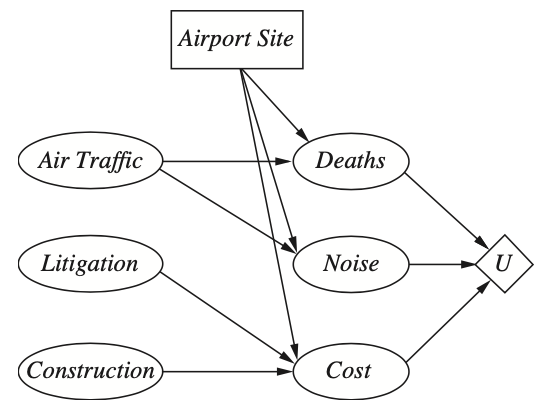
\includegraphics{images/decision-network.png}
    \caption{A simple decision network for the airport-siting problem}
    \label{fig:dn}
\end{figure}

A simplified form is also used in many cases. The notation remains identical, but the chance nodes describing the outcome states are omitted. Instead, the utility node is connected directly to the current-state nodes and the decision node. This representation allows us to expression the utility function that is \textit{conditioned} directly on the immediate factors(current-state nodes), and the action decided at the decision nodes. This is analogous to the \textbf{$Q$-function} or the \textbf{action-utility function}. By omitting intermediate outcomes node, we have a more explicit utility function that is expressed over actions.

\subsubsection{Evaluating Decision Networks}

Actions are selected by evaluating the decision network for each possible setting of the decision node. Once the decision node is set, it behaves exactly like a chance node that has been set as an evidence variable, since we have fixed the value of the decision node based on the action we choose at this node. The general algorithm is as follows:

\begin{enumerate}
    \item Set the evidence variables for the current state.
    For each possible of the decision node:
    \begin{enumerate}
        \item Set the decision node to that value.
        \item Calculate the posterior probabilities for the parent nodes of the utility node, using the standard probabilistic inference algorithm on Bayesian networks.
        \item Calculate the resulting expected utility for that action using the posterior probabilities computed at the parent nodes of the utility node.
    \end{enumerate}
    \item Return the action with the highest utility.
\end{enumerate}

\subsection{Value of Information}
In preceding analysis, we have assumed that all relevant information that is available is provided to the agent before it makes a decision. In practice this is hardly ever the case, and hence \textit{one of the most important parts of decision making is knowing what questions to ask}. In this section, we will describe \textbf{information value theory}, which enables an agent to choose what information to acquire next. We also make the assumption that the agent can acquire the value of any potentially observable chance variables in the model.\\

Let us begin with an example: Suppose an oil company is hoping to buy one of $n$ indistinguishable blocks of ocean-drilling rights. We further assume that exactly one of the blocks contains oil worth $C$ dollars, while the others are worthless. The asking price of each block is $\frac{C}{n}$ dollars. If the company is risk neutral, then it will be indifferent between buying a block and not buying one, since:

$$
EU(Buy) = \frac{1}{n}(C) - \frac{C}{n} = 0
$$
$$
EU(NoBuy) = 0
$$

Now, supposed that a seismologist offers the company the results of a survey of block number 3, which indicate whether the block contains oil. How much should the company be willing to pay for such information? That is, how much is the information worth? We can analyse this by looking at the expected profit given this information:

\begin{itemize}
    \item With probability $\frac{1}{n}$, the survey will indicate oil in block 3. In this case, the company will buy the block for $\frac{C}{n}$ dollars and make a profit of $C - \frac{C}{n} = (n-1)\frac{C}{n}$ dollars.
    \item With probability of $\frac{n-1}{n}$, the survey will show the block has no oil. In this case, the company will then buy a different block. The probability of finding oil in one of the other blocks changes from $\frac{1}{n}$ to $\frac{1}{n-1}$, so the expected profit the company makes is $\frac{1}{n-1}C - \frac{C}{n} = \frac{C}{n(n-1)}$.
\end{itemize}

Using the above information, we calculate the expected profit, given the survey information:

$$
\frac{1}{n}[(n-1)\frac{C}{n}] + \frac{n-1}{n}[\frac{C}{n(n-1)}] = \frac{C}{n}
$$

Hence, the value of this survey information is $\frac{C}{n}$, or also that the company should not be willing to pay more than $\frac{C}{n}$ dollars for this information since the expected profit is $\frac{C}{n}$.

\subsubsection{General formula for Perfect Information}

Given our initial assumption that the exact evidence can be obtained about the value of some random variable $E_j$ for all observable variables, we can derive the general mathematical formula for the value of information. Let the agent's initial evidence be $e$. Then, the value of the current best action $\alpha$ is defined by:

$$
EU(\alpha | e) = \underset{a}{\max} \sum_{s'} P(\textsc{RESULT}(a)=s'|a, e) U(s')
$$

Next, we are now interested in the \textit{value of information} provided by some new evidence $E_j = e_j$; That is, after observing $E_j = e_j$, how much does this evidence contribute to the new value of the best action?

$$
EU(\alpha_{e_j} | e, e_j) = \underset{a}{\max} P(\textsc{RESULT}(a)=s'|a, e, e_j) U(s')
$$

Since $E_j$ is a random variable whose value is currently unknown, to determine the value of discovering $E_j$, we need to account for all possible realizations of $E_j$ by marginalizing over all values of $E_j$ using our \textit{current beliefs} about it's value to obtain the \textbf{Value of Perfect Information}(VPI):

$$
VPI_e(E_j) = \left( \sum_k P(E_j = e_{jk} | e) EU(\alpha_{e_{jk}} | e, E_j = e_{jk}) \right) - EU(\alpha | e)
$$

Intuitively, we can think of the VPI as measuring the expected increase in our expected utility from discovering the random variable $E_j$. This is analogous to information gain in decision trees.

\subsubsection{Properties of Value of Information}

The VPI of any random variable $E_j$ has the following properties:

\begin{itemize}
    \item \textit{The expected value of information is non-negative}.
    $$
    \forall e, E_j, VPI_e(E_j) \geq 0
    $$
    
    Intuitively, we can expect this to hold: If the information results in a worse utility than before, we can simply ignore the information as we can merely take the best action from before $E_j$ was discovered.
    
    \item \textit{VPI is not additive.}
    $$
    VPI_e(E_j, E_k) \neq VPI_e(E_j) + VPI_e(E_k)
    $$
    
    Since VPI depends on the current state of information, it's evaluation on a random variable $E_j$ can go up or down if another random variable $E_k$ is discovered as well, since the value of $E_k$ could potential affect the value of $E_j$ sampled after $E_k$, based on how the information from $E_k$ influences the information of $E_j$.
    
    \item \textit{VPI is order independent.}
    $$
    VPI_e(E_j, E_k) = VPI_e(E_j) + VPI_{e, e_j)}(E_k) = VPI_e(E_k) + VPI_{e, e_k}(E_j)
    $$
\end{itemize}

 \subsubsection{Information Gathering Agents}

A sensible agent should ask questions in a reasonable order, should avoid asking questions that are irrelevant, should take into account the importance of each piece of information in relation to its cost, and should stop asking questions when that is appropriate. All of these capabilities can be achieved by using the value of information as a guide.\\

We now introduce a general algorithm for a rational agent that gathers information by querying information that provides the greatest value. Each random variable $E_j$ is associated with a cost $Cost(E_j)$ that reflects the cost of obtaining the evidence of $E_j$. If the value of a random variable is desirable, the agent can query for it using the $\textsc{REQUEST}(E_j)$ procedure.\\

\begin{algorithmic}
\Procedure{\textsc{Information-Gathering-Agent}}{$percept$} \Return an $action$
\State \textbf{persistent:} $D$, a decision network\\

\State integrate $percept$ into $D$
\State $j \leftarrow$ the value that maximizes $\frac{VPI_e(E_j)}{Cost(E_j)}$
\If{$VPI_e(E_j) > Cost(E_j)$}
\State \Return \textsc{Request}$(E_j)$
\Else \Return the best action from $D$
\EndIf

\EndProcedure
\end{algorithmic}

The agent algorithm that we have described implements a \textbf{myopic} form of information gathering; That is, it uses the VPI formula shortsightedly by calculating the value of information as if only a single evidence variable will be acquired, instead of accounting for future evidences.

\pagebreak
\section{Markov Decision Processes}

Previously, we have dealt with planning actions in a \textit{deterministic} environment, where we formulated a plan of actions that allowed us to get from initial state to the goal. In the case of stochastic environments uncertainty is involved, such methods is not possible as an optimal sequence of actions in a deterministic setting may not always lead us to the goal state in a stochastic one due to uncertain effects in the process of performing actions.

\subsection{Sequential Decision Problems}

Because of the inherent uncertainty present in stochastic environments, we need to \textit{observe} the outcomes whenever we perform an action. For example, consider the situation where we are driving on the road, and we have no information on traffic congestion. If we observe that traffic in the roads far ahead is jammed, then we may consider taking a detour or alternative route. Else, we can just proceed with the straight path. As such, we now model the problem as a \textbf{sequential decision problem}, where we sequentially choose actions to perform based on our current state.\\

In particular, we model sequential decision problems as a \textbf{Markov Decision Process}(MDP) with a transition model $T$ that defines a \textit{probability distribution} over possible outcomes, denoted as $P(s'|s, a)$ conditioned on the action $a \in A$ taken at state $s$ due to the stochasticity over outcomes. Furthermore, by virtue of the namesake of MDP, we assume a Markovian property over transitions where the probability of the next state $s'$ is only dependent on the current state $s$ and none of the states before that. This simplifies our problem as we do not need to maintain a history of actions and states. Additionally, each state $s$ is also associated with a reward $R(s)$, which we shall see later that correlates to the utility of the state $s$.\\

In a nutshell, a sequential decision process for a fully observable stochastic environment with a Markovian transition model and additive rewards is called a Markov Decision Process, and consists of a set of states with initial state $s_0$, a set of actions $A$ in each state, a transition model $P(s' | s, a)$ and a reward function $R(s)$.\\

We have seen that a fixed sequence of actions cannot necessarily be the solution due to stochasticity involved. Instead, the solution for MDPs is known as a \textbf{policy}, which is a function $\pi(s)$ that specifies what action an agent should take in a state $s$. Additionally, we also cannot determine the exact value or utility of a sequence of actions generated by a policy $\pi$, since outcomes are unknown until they happen. We then measure the quality of a policy by the \textit{expected utility} over possible environment histories that can be generated by the policy $\pi$. An optimal policy is one that yields the highest possible expected utility, and is denoted by $\pi^*$. Given this optimal policy $\pi^*$, the agent determines what actions $a = \pi^*(s)$ to take by consulting the policy. 

\subsection{Utilities over time}

In sequential decision problems, utilities no longer depend on episodic outcomes as in the previous section on decision theory, but over the entire environment history generated. \\

First we ask the question of whether the problem is a \textbf{finite horizon} one, or \textbf{infinite horizon}. Finite horizon problems usually only have a fixed number of actions to perform. That is, there is a \textit{fixed} time $N$ after which nothing matters. More formally, $U_h([s_0, \cdots, s_{N+k}]) = U_h(s_0, \cdots, s_{N})$ for all $k > 0$. Another way to interpreting this is that \textit{the optimal action in a given state could change over time}. We say that such a policy in such a situation is \textbf{non-stationary}: Optimal action at a state depends on time as well. In finite horizon planning problems, it is often likened to an approximate search problem using a search tree.\\

On the other hand, in infinite horizon problems, the search could theoretically go on for as long as possible, and there is (infinitely) as much time left after executing each action. Hence, there is no reason to behave differently at different times given the same state, and the optimal policy is \textbf{stationary}. Very often, policies for infinite horizon problems are therefore easier to deal with since we don't need to handle the concept of time. As such, as shall mainly deal with infinite horizon planning problems in this section.\\

Given stationarity, it turns out that it is not too difficult to define utilities over a environment history generated via a sequence of actions.

\begin{enumerate}
    \item \textbf{Additive rewards}. The utility of a state sequence is simply the sum of rewards of each state in the environment history.
    
    $$
    U_h([s_0, s_1, \cdots]) = R(s_0) + R(s_1) + \cdots
    $$
    
    However, it is obvious that given an infinite horizon setting, using a summation can result in rewards that stretch out to infinity! Instead, we use the second method of assigning utilities:
    
    \item \textbf{Discounted rewards}.
    
    $$
    U_h([s_0, s_1, \cdots]) = R(s_0) + \gamma R(s_1) + \gamma^2 R(s_2)+ \cdots
    $$
    
    where the \textbf{discount factor} $0 \leq \gamma \leq 1$ acts as a weight decay for subsequent rewards after the next immediate state. The discount factor represents the importance of immediate rewards over future rewards, and also the preference of future over current rewards. Values of $\gamma$ closer to 0 indicates that the agent is myopic and only focuses on immediate rewards, while those closer to 1 indicates that future rewards are as significant as immediate ones. Another interesting observation is that this is generalization over the additive rewards when the discount factor $\gamma = 1$, hence without loss of generality, we can stick to using the discounted reward scheme over the additive one.
\end{enumerate}

Now, we turn to details associated with the problem of infinite horizon planning: Dealing with possibly infinitely long sequences of actions. To handle this issue, we look at the following properties:

\begin{enumerate}
    \item With discounted rewards, it can be shown that the utility of an infinite sequence if \textit{finitely bounded} for when $\gamma < 1$. Furthermore, if we assume that the rewards $R(s)$ are bounded by $\pm R_{\max}$, we have:
    
    $$
    U_h([s_0, s_1, \cdots]) = \sum^{\infty}_{t=0} \gamma^t R(s_t) \leq \sum^{\infty}_{t=0} \gamma^t R_{\max} = \frac{R_{\max}}{1-\gamma}
    $$\
    
    where the last part is obtained by applying the standard formula for an infinite geometric series.
    
    \item Infinite sequences can also be compared in terms of the \textbf{average reward} obtained per time step:
    
    $$
    U_h([s_0, s_1, \cdots]) = \lim_{T \rightarrow \infty} \frac{1}{T}(R(s_0) + R(s_1) + \cdots)
    $$
    
    However, such cases are generally harder to handle mathematically.
    
\end{enumerate}

\subsection{Optimal Policies and Utilities of states}

Having decided that the utility of a given state sequence is the sum of discounted rewards obtained during the sequence, we can compare utilities by comparing expected utilities of policies to elicit preferences of policies according to decision theory. The expected utility of a policy $\pi$ starting in state $s$ is given by:

$$
U^{\pi}(s) = \mathbb{E} \left[ \sum^{\infty}_{t=0} \gamma^t R(S_t) \right]
$$

where the expectation is with respect to the probability distribution over the state sequences determined by $\pi$ and $s$. Using the above expected utility, according to decision theory a rational agent would select the optimal policy $\pi^*$ that corresponds to the maximum utility over other policies $\pi$ using the above utility.

$$
\pi^*_s = \underset{\pi}{\arg\max} U^{\pi}(s) 
$$

Where $\pi^*_s$ is the optimal policy starting in state $s$. By stationarity of infinite horizon planning, we have that the optimal policy starting at state $s$ is equivalent to the optimal policy $\pi^*$ regardless of the starting state $s$.

\subsection{Value-Iteration}

\subsubsection{Bellman Equations for Utilities}

From the previous section and decision theory, the utility function $U(s)$ allows the agent to selections by principle of maximum expected utility. That is, we want our optimal policy to choose the best action the maximizes the expected utility of the subsequent state.

$$
\begin{aligned}
\pi^*(s) &= \underset{a \in A(s)}{\arg\max} U^{\pi}(s)\\
&= \underset{a \in A(s)}{\arg\max} \left( R(s) + \gamma R(T(s, \pi(s)) + \cdots \right)\\
&= \underset{a \in A(s)}{\arg\max} \left(R(T(s, \pi(s)) + \cdots \right)\\
&= \underset{a \in A(s)}{\arg\max} \left( \mathbb{E}[U^{\pi}(s')] \right)\\
&= \underset{a \in A(s)}{\arg\max} \sum_{s'} P(s' | s, a) U(s')
\end{aligned}
$$

Then, the utility following the principle of maximum expected utility is as follows:

$$
\begin{aligned}
U(s) &= \max_{\pi} U^{\pi}(s)\\ 
&= \max_{\pi}\left( R(s) + \gamma R(T(s, \pi(s)) + \cdots \right)\\
&= R(s) + \gamma \max_{\pi}\left(R(T(s, \pi(s)) + \cdots \right)\\
&= R(s) + \gamma \max_{\pi}\left( \mathbb{E}[U^{\pi}(s')] \right)\\
&= R(s) + \gamma \underset{a \in A(s)}{\max} \sum_{s'} P(s' | s, a) U(s')
\end{aligned}
$$

that gives the following explanation: \textit{The utility of a state is the immediate reward for that state plus the expected discounted utility of the next state, assuming that the agent chooses the optimal action}.

\subsubsection{Value-Iteration algorithm}

An issue with the above equations is that the introduction of the $\max$ operator induces \textit{non-linearity}. As a result, we cannot easily solve them using a system of linear operations. Instead, we try an \textit{iterative} approach to solving it by initializing arbitrary values to the utility of each state, and then repeatedly updating the utilities. Let $U_i(s)$ be the utility value for state $s$ at the $i^{th}$ iteration, then the iterative step is as follows:

$$
U_{i+1}(s) \leftarrow R(s) + \gamma \underset{a \in A(s)}{\max} \sum_{s'} P(s' | s, a) U_i(s')
$$

which is also known as the \textbf{Bellman update} equation. This update equation is the essence of the value iteration algorithm.

\begin{algorithm}[!htb]
\caption{\textsc{Value-Iteration}}
\begin{algorithmic}[1]
\Procedure{\textsc{Value-Iteration}}{$mdp, \epsilon$} \Return a utility function
\State \textbf{Input:} \\
\hspace*{\algorithmicindent} \hspace*{\algorithmicindent} $mdp$, an MDP with states $S$, actions $A(s)$, transition model $P(s' | s, a)$,\\ 
\hspace*{\algorithmicindent} \hspace*{\algorithmicindent} rewards $R(s)$ and discount $\gamma$\\ 
\hspace*{\algorithmicindent} \hspace*{\algorithmicindent} $\epsilon$, the maximum error allowed in the utility of any state

\State \textbf{Local variables:} \\
\hspace*{\algorithmicindent} \hspace*{\algorithmicindent} $U, U'$, vectors of utilities for states in $S$, initially zero\\
\hspace*{\algorithmicindent} \hspace*{\algorithmicindent} $\delta$, the maximum change in the utility of any state in an iteration\\

\Repeat
\State $U \leftarrow U'; \delta \leftarrow 0$

\For{state $s \in S$}
\State $U'[s] \leftarrow R(s) +  \gamma \underset{a \in A(s)}{\max} \sum_{s'} P(s' | s, a) U[s']$
\If{$|U'[s] - U[s]| > \delta$}
\State $\delta \leftarrow ||U'[s] - U[s]|$
\EndIf
\EndFor

\Until{$\delta < \frac{\epsilon(1-\gamma)}{\gamma}$}

\EndProcedure
\end{algorithmic}
\end{algorithm}

\subsubsection{Convergence of Value-Iteration}

What is interesting about the value-iteration algorithm we have seen, is that it \textit{eventually converges} to a unique set of solutions of the Bellman equations. The key concept in showing why this is so is the notion of \textbf{contraction}. Contraction in the intuitive sense, is a function of one argument that when applied to two different inputs in turn, produces two output values that have smaller differences by at least some constant factor then the original inputs. We then discern the following properties of contractions:

\begin{itemize}
    \item A contraction has only one fixed point; That is, a point where applying the function does not change it's value. If there were two fixed points, applying the function to both points do not yield outputs that are 'closer' together, contradicting the definition of contraction.
    \item When the function is applied to any argument, the value must get closer to the fixed point(because the fixed point does not change), so repeated application of a contraction always reaches the fixed point in limit.
\end{itemize}

Now, suppose we view the Bellman update as an operator $B$ that is applied simultaneously to update the utility of every state. Let $U_i$ denote the vector of utilities for all the states at the $i^{th}$ iteration. Then, then Bellman update equation can be written as follows:

$$
U_{i+1} \leftarrow BU_i
$$

Next, to measure the distances of utility vectors, we make use of the \textbf{max norm} or infinity norm, that measures the value of a vector the maximum value that appears in any element in the vector - The absolute value of it's biggest component.

$$
|U|_{\infty} = \max_s |U(s)|
$$

With this definition, the 'distance' between vectors $|U - U'|_{\infty}$ is the maximum difference between any two corresponding elements. We now first show that $B$ is indeed a contraction. Before we do so, we make the following observation:

$$
\begin{aligned}
U_{i+1}(s) &\leftarrow R(s) + \gamma \underset{a \in A(s)}{\max} \sum_{s'} P(s' | s, a) U_i(s')\\
&= (R + \gamma \underset{a \in A(s)}{\max}\sum_{s'} TU_{i})(s)
\end{aligned}
$$

is represented in the form of a system of vectors and matrices, and $U_{i+1}, U_i$ are vectors representing state values, where:

\begin{itemize}
    \item $R$ represents the reward vector over states
    \item $T$ is a transition matrix containing probabilities when the optimal policy $\pi^*$ is followed
    \item $U_{i+1}, U_i$ are utility vectors containing the utilities of each state at time $i+1, i$ respectively
\end{itemize}

Then, let $U$ be the vector containing the \textit{true} utilities of each state. As such, it is also a fixed point for the contraction $B$ since the utilities cannot go higher than this true optimal utilities. Then, we have that at time $i$:

$$
\begin{aligned}
\left| U_{i+1} - U \right|_{\infty} & = \left| BU_{i} - U \right|_{\infty}\\
&= \left| BU_i - BU \right|_{\infty} \text{ (by definition of fixed point: $BU = U$)}\\
&= \left| R + \gamma TU_i - (R + \gamma TU) \right|_{\infty}\\
&= \left| \gamma \underset{a \in A(s)}{\max} TU_i  - \gamma \underset{a \in A(s)}{\max} TU \right|_{\infty}\\
&leq \gamma \underset{a \in A(s)}{\max} \left| T(U_i  - U) \right|_{\infty}\\
&\leq \gamma \underset{a \in A(s)}{\max} \left| T \right|_{\infty} \left| (U_i  - U) \right|_{\infty} \text{ (Using Cauchy-Schwartz inequality)}\\
&\leq \gamma \left| (U_i  - U) \right|_{\infty}
\end{aligned}
$$

Where we used the following result that:

$$
\begin{aligned}
\left| \max_a f(a) - \max_a g(a) \right| &= \left| f(a') - \max_a g(a) \right| \text{ where } a' = \arg\max_a f(a) \\
&\leq \left| f(a') - g(a') \right|\\
&\leq \max_a |f(a) - g(a)|
\end{aligned}
$$

which says that individually difference of two individually maximized terms is no more than the maximization of the difference of the two terms together. The last line results from the fact that the maximum over the transition probability matrix over the actions $a$, gives a probability matrix of the optimal policy. Multiplying this transition matrix over the utility values difference, is an \textit{expectation} over the difference in utility values given this distribution. This is a convex combination of values of the original difference $(U_i  - U)$, and cannot increase the maximum difference between utilities of any state $s$.\\

Finally, we have shown that the Bellman update operator $B$ is indeed a contraction. Then, by repeatedly applying the contraction, we get that:

$$
\begin{aligned}
|U_t - U|_{\infty} &= |BU_{t-1} - U|_{\infty}\\
&\leq \gamma |U_{t-1} - U|_{\infty} \text{ (By contraction of $B$)}\\
&\leq \gamma^t |U_0 - U|_{\infty}
\end{aligned}
$$

If we view $|U_0 - U|_{\infty}$ as the error estimate on the true utilities $U$, then given that the discount factor $\gamma < 1$, this error is reduced by a factor of $\gamma$ each time, and becomes smaller. The value iteration hence converges exponentially fast. Furthermore, we can compute the number of iterations required for convergence. Recall that we make the assumption that the values of states are bounded by $\pm \frac{R_{\max}}{1 - \gamma}$. Then, the initial error is bounded by $|U_0 - U|_{\infty} \leq \pm 2\frac{R_{\max}}{1 - \gamma}$. Let $N$ denote the number of iterations that is required to reach an error of $\epsilon$ at most. Then, with a bit of manipulation we get that:

$$
\gamma^N \cdot 2\frac{R_{\max}}{1 - \gamma} \leq \epsilon \implies N = \frac{\log(2\frac{R_{\max}}{1 - \gamma})}{\log(N)}
$$

This brings us to the terminating condition of value-iteration comes from the fact that $|U_{i+1} - U_i|_{\infty}  \leq \frac{\epsilon (1-\gamma)}{\gamma}\implies |U_{i+1} - U|_{\infty} \leq \epsilon$.

\subsection{Policy-Iteration}

In the previous section, we observed though it is possible to get an optimal policy even when the utility function estimate is inaccurate through the fixed point iteration. We follow up with the observation that is one action is clearly better than the other, the exact magnitude of the utilities on the states involved need not be precise if the selection of the action is still selected by the policy. This insight suggests an alternative way to find optimal policies, which is described as \textbf{policy iteration}. Policy iteration alternates between the following two steps to obtain the optimal policy:

\begin{itemize}
    \item \textbf{Policy Evaluation:} Given a policy $\pi_i$, calculate the utility of the states according to the current policy $U_i = U^{\pi}_i$ for each state we execute actions by following the policy $\pi_i$.
    \item \textbf{Policy Improvement:} Calculate a new maximum expected utility policy $\pi_{i+1}$ using one-step look-ahead based on $U_i$.
\end{itemize}

The algorithm terminates when the policy improvement step yields no change in utilties. At this point, while the utilities may not be the optimal utility function, the utility function $U_i$ is a fixed point over the policy $\pi_i$ since improving on the utility functions via value-iteration would not yield a different policy. Given that there are finite number of policies for finite state spaces, the policy-iteration algorithm will eventually terminate.\\

A question that we wish to ask next is how do implement the policy evaluation routine to find out the utilities of states? It turns out that the equation for doing so is relatively similar and simplified version of the Bellman equations that we have seen before:

$$
U_i(s) = R(s) + \gamma \sum_{s'} P(s' | s, \pi_i(s)) U_i(s')
$$

that represents the utility of a state $s$ by following policy $\pi_i$. Notice that now the $\max$ operator is not present unlike in the case of value-iteration. Since the policy evaluation equations are linear, the system of linear equations representing the utilities over all states can be solved using linear algebra methods, which incurs $O(n^3)$ time for a state space of $n$ states. For cases where $n$ is large, this time complexity may be expensive, and we can perform iterative update of the above equation as we did in value-iteration. The algorithm for policy iteration is as follows:

\begin{algorithm}[!htb]
\caption{\textsc{Policy-Iteration}}
\begin{algorithmic}[1]
\Procedure{\textsc{Policy-Iteration}}{$mdp$} \Return a policy
\State \textbf{Input:} \\
\hspace*{\algorithmicindent} \hspace*{\algorithmicindent} $mdp$, an MDP with states $S$, actions $A(s)$, transition model $P(s' | s, a)$,\\ 

\State \textbf{Local variables:} \\
\hspace*{\algorithmicindent} \hspace*{\algorithmicindent} $U$, vectors of utilities for states in $S$, initially zero\\
\hspace*{\algorithmicindent} \hspace*{\algorithmicindent} $\pi$, policy 
vector indexed by state, initially random\\

\Repeat
\State $U \leftarrow \textsc{Policy-Evaluation}(\pi, U, mdp)$
\State $unchanged? \leftarrow \text{true}$

\For{state $s \in S$}
\If{$\underset{a\in A(s)}{\max} \sum_{s'} P(s' | s, a) U[s'] > \sum_{s'} P(s' | s, \pi[s]) U[s']$}
\State $\pi[s] \leftarrow \underset{a \in A(s)}{\arg\max} \sum_{s'} P(s' | s, a) U[s']$
\State $unchanged? \leftarrow \text{false}$
\EndIf
\EndFor

\Until{$unchanged?$}

\EndProcedure
\end{algorithmic}
\end{algorithm}

In the policy iteration, we iteratively update the policy $\pi$ with the best action $a$ over each state $s$, then following the policy from the next state onwards. This reflects the one step look-ahead that we have mentioned before, where we consider the rewards of each action and the utility of the state one-step ahead of $s$. This update step is similar to the iterative update step from the value-iteration algorithm.

\subsubsection{Policy Improvement Theorem}

The correctness of the policy-iteration algorithm follows the \textbf{policy improvement theorem}, which is defined as the following.

\begin{theorem}
Let $Q^{\pi}(s, a) = R(s) + \gamma \sum_{s'} P(s' | s, a) U^{\pi}(s')$ be the action-value function for $\pi$. Let $\pi, \pi'$ be any pair of deterministic policies such that for all $s \in S$,
$$
Q^{\pi}(s, \pi'(s)) \geq Q^{\pi}(s, \pi(s)) = U^{\pi}(s)
$$

Then, $U^{\pi'}(s) \geq U^{\pi}(s)$ for all $s\in S$.
\end{theorem}

\textbf{Proof.} Given that $Q^{\pi}(s, \pi'(s)) \geq U^{\pi}(s)$, we have that:

$$
\begin{aligned}
U^{\pi}(s) &\leq Q^{\pi}(s, \pi'(s))\\
&= R(s) + \gamma \sum_{s'} P(s' | s, \pi'(s)) U^{\pi}(s')\\
&= \mathbb{E}_{\pi'}[R(S^t) + \gamma U^{\pi}(S^{t+1}) | S^t = s]\\
&\leq \mathbb{E}_{\pi'}[R(S^t) + \gamma \mathbb{E}_{\pi'}[Q^{\pi}(S^{t+1}, \pi'(S^{t+1}))] | S^t = s]\\
&= \mathbb{E}_{\pi'}[R(S^t) + \gamma \mathbb{E}_{\pi'}[R(S^{t+1}) + \gamma U^{\pi}(S^{t+2})] | S^t = s]\\
&= \mathbb{E}_{\pi'}[R(S^t) + \gamma R(S^{t+1}) + \gamma^2 U^{\pi}(S^{t+2}) | S^t = s]\\
&\leq \mathbb{E}_{\pi'}[R(S^t) + \gamma R(S^{t+1}) + \gamma^2 R(S^{t+2}) + \cdots | S^t = s]\\
&= U^{\pi'}(s)
\end{aligned}
$$

The implication of this theorem is that we can replace our current policy $\pi$ with another $\pi'$, if the utility of $\pi'$ is never below that of $\pi$. Tying this to policy iteration, Each update step of the policy changes a single action indexed in the policy $\pi$ to the action that gives the maximum utility. Hence, the policy perturbs an action of the policy at each update step, and at each step, the utility of each stage according to the updated policy \textit{can only improve}. Hence, the policy eventually converges to an optimal one by the policy improvement theorem.

$$
U^{\pi'}(s) \geq \underset{a \in A(s)}{Q^{\pi}(s, a)} \geq Q^{\pi}(s, a) = U^{\pi}(s)
$$

Where the first inequality is derived from the fact there may be compounded improvements. 

\section{Online Search}

In many problems, the state space is very large and often grows exponentially with the number of variables. This causes policy iteration and value iteration algorithms to be intractable, as they iterate through each of the states during the update steps. Many methods have been introduced to address this, the most popular now being using function approximation through deep neural networks. Another common method is through sampling. In this section, we shall look at sampling based methods in what is known as \textbf{online search}.\\

In online search under the stochastic environment, we often construct a search tree up to a fixed depth of $D$. We represent the current state as the root node, and the nodes in the tree are separated into \textit{observation nodes} and \textit{action nodes}. Action nodes represent the current state and encapsulate \textit{states} in the state space. Edges of the action nodes each represent an action that can be taken at the state $s$ at the action node, and children of these edges are observation nodes that capture information of the observation after taking the action.\\

On the other hand, observation nodes captures the results of taking an action $a$, and edges from these nodes lead to action nodes that encapsulate possible outcomes of taking the action $a$ from state $s$. The edges represents the reward $z_i$ of getting to outcome $i$. The stochasticity is inherently captured in the form of a probability distribution over each of the edges and outcomes. \\

At observation nodes, we take the expectation over the utility of each possible outcome just as we did in an MDP using weighted averages over the probability distribution on outcomes, and at action nodes we take the maximum over the expected utilities at observation nodes.\\

\begin{figure}[!htb]
    \centering
    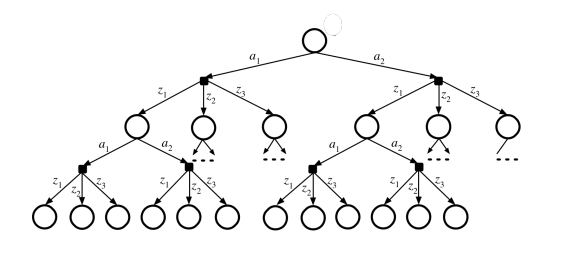
\includegraphics[width=8cm]{images/online-search-tree.png}
    \caption{Naive online search tree}
\end{figure}

However, observe that even with such a setting by limiting the depth $D$, we still have not addressed the issue of exponentially increasing state space. This is because at each of the observation nodes, it branches out into $|S|$ nodes for each of the possible outcomes in the state space. Then, the search tree size is $|A|^D|S|^D$ and is still grows very quickly. Instead, we can make use of \textit{sampling} to reduce the branching factor at observation nodes. Given that we have a probability distribution at observation nodes, we can sample $k$ outcomes from this probability distribution instead of using all $|S|$ states where $k << |S|$. This reduces the tree size to $|A|^D k^D$.

\subsection{Rollout}

However, let us now assume we have a policy $\pi$, that could be possibly obtained from value iteration or policy iteration. Then, our objective is to improve upon such a policy(that may not be optimal) in an exponentially large state space. We again employ the use of sampling to do this.

\textbf{Rollouts} does this by assuming a current state $s$ and a policy $\pi$. Then, we estimate the state-action function $Q(s, a)$ at $s$ by simulating many trajectories from $s$ using each action $a$, where the simulations following the action $a$ are done using $\pi$. We then select the action $a = \underset{a \in A(s)}{\arg\max} Q(s, a)$ with the highest return or utility.\\

Similar to the update step in policy iteration, rollouts aims to obtain an improved utility estimate at a state $s$ by considering all actions $a$ at state $s$, then estimating the value of the subsequent state $s'$ of taking the action $a$ by using multiple trajectories following the policy $\pi$. Hence, by the policy improvement theorem and assuming that the policy estimates are accurate enough, the improved utility values at $s$ is a better estimate or improvement on the utility estimate using $\pi$ since it is analogous to the update step in policy iteration. In particular, rollouts can be said to produce an even more accurate update that in policy iteration, since we obtain multiple samples per action and simulate the trajectory to obtain it's actual utilities.

\subsection{Monte-Carlo Tree Search}

As mentioned before, with state spaces that are large, the search tree also increases exponentially with the size of the state space. The \textbf{Monte-Carlo Tree Search}(MCTS) addresses this issue by only expanding promising nodes, and using sampling to estimate the utility of a node that has previously not been discovered. The use of sampling techniques helps to alleviate the issues associated with exponentially growing tree sizes.\\

The MCTS framework repeatedly runs trials from the root node, where a trial either repeatedly selects a node to go to at the next level until target depth is reached, or uses a rollout policy on the node if it has not yet been discovered. For specifically, the MCTS framework consists of the following procedures:

\begin{itemize}
    \item \textbf{Selection:} Starting at the root node, traverse down the search tree by repeatedly selecting the node that looks most promising, until a leaf node is reached or the current node has not yet been fully expanded.\\
    
    The notion of 'promising' is a configurable component that can be decided by the user, and will be elaborated further in a later section.\\
    \item \textbf{Expansion:} We expand out an unexplored child node that has not yet been evaluated before.\\
    
    \item \textbf{Simulation:} We then evaluate the return at the newly expanded child node by running simulations on it. This is again a configurable component where different simulation techniques may be employed. In this setting, we assume that the rollout policy is used in simulation.\\
    
    \item \textbf{Backup:} We then update the information of the simulations performed at this node, and also propagate the information about this node up the tree of the nodes traverse along the current path from the root.
\end{itemize}

It is useful to note that MCTS is an \textit{anytime} policy: It performs as many iterations of the framework as possible, then returns the best action at the root node when the budget or time is fully expended. As such, MCTS aims to collect as much information as possible through the use of sampling in order to estimate the utilities of each action accurately.\\

In the case where we perform online planning using MCTS on an MDP, we have the following:

\begin{itemize}
    \item In the search tree, each node $n$ is associated with a state $s$ in the state space.
    \item The next node $n'$ at the next level is selected by applying an action $a$ to the current state $s$, then sampling the next state $s'$ according to the probability distribution $P(s' | s, a)$.
    \item The estimated value $\hat{V}(n)$ at a node $n$ is the average return of all the trials at $n$, where the return $r_t(n)$ of trial $t$ starting from $n$ with state $s$ and next node $n'$ is given by:
    $$
    r_t(n) = R(s) \gamma r_t(n')
    $$
    
    Then, the estimated state-action value $\hat{Q}(n, a)$ at $n$,is the average return of all trials run from $n$ the starts by taking the action $a$.
\end{itemize}

\subsubsection{Node Selection}

In selecting children nodes, we mentioned that we wish to select children nodes that are \textit{promising}. However, how do we define the notion of promising nodes? One way that we have seen is to select children nodes that maximize the expected utility. That is, we follow the theory of utility by maximizing the value $U(s) = \max Q(s, a)$. However, in doing so we select actions in a deterministic manner. This is similar to the multi-armed bandit problem, where an adversary can devise inputs that causes MCTS to perform very badly. Additionally, MCTS is a form of \textit{asymmetric} tree search, we do not expand out all the nodes, and hence may not have sufficient information on all paths. This is important, because we may essentially miss paths along unexplored children nodes that may lead to optimal utilities! This is known as \textbf{exploration}.\\

As such, we want to improve on the greedy strategy of the following:

$$
\pi(n) = \underset{a \in A(s)}{\arg\max} \hat{Q}(s, a)
$$

We also wish to trade-off between exploration of unvisited nodes in hopes of discovering better utilities, and exploiting the information we currently have to get to states that we know have the best returns. There are many formulations that aim to do this, but by far the most popular is the \textbf{Upper-Confidence Bound}(UCB) algorithm. In particular, we look at the search-tree variant of UCB known as \textbf{Upper-Confidence Tree}(UCT), which is formulated as the following:

$$
\pi_{UCT}(n) = \underset{a \in A(s)}{\arg\max} \left( \hat{Q}(s, a), c \sqrt{\frac{\log(N(n))}{N(n, a)}} \right)
$$

where:

\begin{itemize}
    \item $N(n)$ is the number of trials performed in the search tree that runs through node $n$.
    \item $N(n, a)$ is the number of trials performed in the search tree through node $n$, followed by taking the action $a$.
\end{itemize}

Here, the second term $c \sqrt{\frac{\log(N(n))}{N(n, a)}}$ is known as the \textit{exploration term}. Intuitively, we can think of this term reflecting the potential of a particular action. If an action $a$ has been taken many times, then the exploration term will be smaller. Conversely, if we do not take action $a$ very often, we may be more incentivized to perform this action to increase our confidence on the returns of this action.

\pagebreak
\section{Reinforcement Learning}

In the previous section, we have seen how we can solve MDPs via \textbf{Value-Iteration} and \textsc{Policy-Iteration}. However, both methods suffer from the issue exploding state space sizes. Instead, we look towards \textit{learning} the optimal policy via \textbf{Reinforcement Learning}.\\

Consider a game of chess. In the case of supervised learning, the agent needs to be explicitly told what is the correct move for each position it encounters. This extremely hard to do so, as enumerating possible state configurations and actions is highly intractable. Instead, the agent receives feedback in the different form known as a \textit{reward}, which is often not received directly and only at the end of the game, such as winning or losing in chess. The notion of rewards have been introduced in the previous section on MDPs, and we continue to build on this notion of the reward function $R$ where the agent aims to maximize it's overall total rewards.

\subsection{Passive Reinforcement Learning}

In passive reinforcement learning, the agent's policy $\pi$ is assumed to be fixed: In state $s$, it always executes the action $\pi(s)$. The goal of the agent is \textbf{to learn how good the policy $\pi$} is, or how good the utility $U^{\pi}(s)$ is. This is highly similar to the \textsc{Policy-Evaluation} routine in the \textsc{Policy-Iteration} algorithm that we have seen before. However, now the main difference is that \textbf{we do not know the transition model $P(s' | s, a)$ nor the reward function $R(s)$}.\\

Hence, the agent first \textit{learns} the model depicted by the transition probabilities $P(s' | s, a)$ and the reward function $R(s)$, and using these learned probabilities and values to compute the utility $U^{\pi}(s)$ using policy-evaluation.

\subsubsection{Direct Utility Estimation}

Direct utility estimation is a \textbf{model-free} reinforcement learning method that aims to learn the utility function values directly. Recall that we do not know the transition model $P(s' | s, a)$ and the reward function $R(s)$. Instead, we bypass this issue by directly estimating the utility values in simulations known as \textbf{trials} to infer the rewards at each of the state in the trajectory during the simulation. As such, this method is also known as \textbf{Monte-Carlo learning}.\\

This method of approximating the utilities of a given state $s$ according the policy $\pi$ known as \textbf{direct utility estimation} uses a simple observation that the utility of a state $s$ is the \textit{expected} total reward from the state onward. Since we do not know the transition probabilities and reward function, we cannot directly compute the utilities of states. However, we can make use of statistical methods to infer such information. \\

Instead, the agent can run a \textit{trial} from it's given state $s$, until the trial ends. Then, the sum of the total rewards for this trial obtained when it terminates is a single \textbf{sample} from the distribution over which the expected utility $\mathbb{E}[U^{\pi}(s)]$ is derived from. Then, by Law of Large Numbers, we can approximate the expected utility $\mathbb{E}[U^{\pi}(s)]$ by doing averaging out the total utility from multiple trials:

$$
\mathbb{E}[U^{\pi}(s)] \approx U_k(s) \frac{1}{k} \sum^k_{n=1} U^{\pi}_n(s)
$$

which approximates the actual expectation well as $k \rightarrow \infty$. It can be seen that direct utility estimation via trials is an instance of supervised learning, where the observation of each trial is used as the output for each input state $s$. As a result, we have reduced reinforcement learning to an inductive learning problem. In fact, the returns at each state at the end of each trial is the \textit{exact} returns at the state under the true probability distribution $P(s' | s, a)$. Hence, the returns of each trial is an unbiased estimate of the expected returns or utility at each state $s$ as well. \\

In many problems, states can be repeated multiple times, and hence there may be multiple copies of states with different rewards in each trial. The choice of using either the \textit{first} visit heuristic to only estimate the value of $U^{\pi}(s)$ with the first visit of state $s$ in a trial, or multiple visits where we make use of every single reward that is obtained when $s$ is visited in a trial is solely left to the user as a design choice.\\

An interesting mathematical result that we can obtain from the average of $k$ returns $G_1(s), \cdots, G_k(s)$ at state $s$ using the estimate $U_k(s)$ of the expected utility of $s$, is that we can rewrite the averaged values over $k$ returns as follows:

$$
\begin{aligned}
U_k(s) &= \frac{1}{k} \sum^k_{i=1} G_i(s)\\
&= \frac{1}{k} \left(G_k(s) \sum^{k-1}_{i=1} G_i(s) \right)\\
&= \frac{1}{k} \left(G_k(s) (k-1) U_{k-1}(s) \right)\\
&= U_{k-1}(s) + \frac{1}{k} \left( G_k(s) - U_{k-1}(s) \right)
\end{aligned}
$$

where $U_{k-1}(s)$ is the estimate of the utility of $s$ after $k-1$ returns, and $G_k(s) - U_{k-1}(s)$ is viewed as the \textbf{prediction error} between the actual return of the $k^{th}$ visit to $s$, and the estimate of the utility of $s$.\\

However, in Monte-Carlo learning, since we perform simulations in the form of trials in order to obtain a sample of the returns at states in the trajectory, we need to finish running each trial completely before we can update all states traversed in the simulation episode. Additionally, as the returns at a state $s$ is a sum of total rewards obtained from successor states and it's own rewards, the variance of such a sum of rewards can be high, and large number of trials may be need to accurately approximate the expected utility at states.\\

\subsubsection{Monte-Carlo Control}

In Monte-Carlo learning or direct utility estimation, we have a fixed policy $\pi$ and we estimate the utility values $U(s)$ using sampling. However, we ultimate want to learn the optimal policy $\pi$ just as in MDPs - This is known as a \textbf{control} problem. We can make use of the idea of \textbf{generalized policy iteration}(GPI) to do so.\\

Recall that in policy-iteration, we repeatedly perform policy-evaluation to compute the current utility estimates with respect to the current policy $\pi$, then make use of the Bellman equations for utility in MDPs to improve the current policy by updating the policy to take the best action over each of the actions at every state. In GPI, we do not know the transition model and reward functions, but we can replicate this 2-stage evaluation and improvement procedure. More specifically, we shall make use of a specific type of utility function known as the \textbf{state-action} utility $Q(s, a)$ that denotes the expected utility of taking the action $a$ at the state $s$. Then, using the principle of maximum expected utility and applying the policy improvement step in \textsc{Policy-Iteration}, we update the policy $\pi$ as:

$$
\pi(s) = \underset{a}{\arg\max} Q(s, a)
$$

to pick the action that maximizes the expected utility from taking any action $a$. It can be seen that this is exactly the same as maximizing our expected utility:

$$
U(s) = \max_a Q(s, a)
$$

And the the Bellman equations for optimality can be rewritten in terms of $Q(s, a)$ and the optimality conditions are still preserved.

$$
Q(s, a) = R(s) + \gamma \sum_{s'} P(s' | s, a) \max_{a'} Q(s', a') = R(s) + \gamma \sum_{s'} P(s' | s, a) U(s')
$$

By formulating utilities in terms of the state-action pair, we implicitly remove the need to learn the transition model and reward functions as they are inherently captured in the utility of the state-action pair itself $Q(s, a)$. Hence, we then follow the similar structure of 2-stage evaluation and improvement procedure as in policy-iteration as follows.

\begin{itemize}
    \item \textbf{Evaluation}. We evaluate the state-action utilities $Q(s, a)$ according to the policy $\pi$ by first performing Monte-Carlo learning to estimate the utilities of each state via samples.\\
    
    To avoid the issue of being stuck in a local optima during Monte-Carlo simulations, we need to balance between exploration and exploitation. We do this by sampling actions in the $k^{th}$ episode/trial by using $\epsilon$-greedy exploration with decaying $\epsilon = \frac{1}{k}$, with respect to being greedy with the current policy $\pi$ and $Q(s, a)$ values. We receive a sequence of returns in each trial: $(S_1, A_1, R_1), \cdots, (S_T, A_T, R_T)$. For each $S_t, A_t$ in the sequence, we do:
    
    $$
    \begin{gathered}
    N(S_t, A_t) = N(S_t, A_t) + 1\\
    Q(S_t, A_t) = Q(S_t, A_t) + \frac{1}{N(S_t, A_t)}(G_t - Q(S_t, A_t))
    \end{gathered}
    $$
    
    where in the second equation, we use the rewritten form of the averaged utilities for MC learning as it's current estimate, plus the prediction error between it and the returns at trial $t$.
    
    \item \textbf{Improvement}. After predicting the utility estimates, we then improve the policy as we did in \textsc{Policy-Iteration} by doing the following step:
    
    $$
    \pi(s) = \underset{a}{\arg\max} Q(s, a)
    $$
    
    which is identical to the improvement step in \textsc{Policy-Iteration} that follows the Bellman conditions for optimality:
    
    $$
    \pi(s) = \underset{a}{\arg\max} R(s) + \gamma \sum_{s'} P(s' | s, a) U(s')
    $$
    
\end{itemize}

We repeat this process multiple times, alternating between the evaluation step using MC learning and the improvement step by being greedy with respect to $Q(s, a)$ to eventually obtain the optimal policy.\\

Nonetheless, this algorithm misses an important source of information that it does not use: The utilities of states are not independent of each other. Under the Bellman equations for MDPs, we have that the \textit{utility of each state equals it's own reward plus the expected utility of it's successor states}. Hence, after updating the utility values for states at the end of each trial, we can use the updated utility values to update utility of predecessor states by switching it's policy to take actions that lead it to the better updated utility. Making use of the constraints imposed by the MDP may also help to address the issue of high variance between returns of different visits to state $s$.

\subsubsection{Adaptive Dynamic Programming}

Adaptive Dynamic Programming(ADP) rectifies the above said issue by taking advantage of the constraints enforced by the Bellman equations for utility in MDPs, by simultaneously solves for the corresponding MDP using dynamic programming to update predecessor states using the utilities of the current. This is achieved used the \textsc{Policy-Evaluation} function as seen in the \textsc{Policy-Iteration} algorithm.\\

The agent that does this called the \textsc{Passive-ADP-Agent}, executes this inductive learning in the algorithm below.

\begin{figure}[!htb]
\begin{algorithmic}[1]
\Procedure{\textsc{Passive-ADP-Agent}}{percept} \Return an action

\State \textbf{inputs}: \\
\hspace*{\algorithmicindent} \hspace*{\algorithmicindent} $percept$, a percept indicating the current state $s'$ and the reward signal $r'$
\State \textbf{persistent}: \\
\hspace*{\algorithmicindent} \hspace*{\algorithmicindent} $\pi$, a fixed policy\\
\hspace*{\algorithmicindent} \hspace*{\algorithmicindent} $mdp$, an MDP with model $P$, rewards $R$ and discount $\gamma$\\
\hspace*{\algorithmicindent} \hspace*{\algorithmicindent} $U$, a table of utilities, initially empty\\
\hspace*{\algorithmicindent} \hspace*{\algorithmicindent} $N_{sa}$, a table of frequencies of state-action pairs, initially zero\\
\hspace*{\algorithmicindent} \hspace*{\algorithmicindent} $N_{s' | sa}$, a table of outcome frequencies given state-action pairs, initially zero\\
\hspace*{\algorithmicindent} \hspace*{\algorithmicindent} $s, a$, the previous state and action, initially null\\

\If{$s'$ is new} $U[s'] \leftarrow r'; R[s'] \leftarrow r'$ \EndIf
\If{$s$ is not null}
\State increment $N_{sa}[s, a]$ and $N_{s' |sa}[s', s, a]$
\EndIf
\For{each $t$ such that $N_{s' | sa}[t, s, a]$ is nonzero}
\State $P(t|s,a) \leftarrow \frac{N_{s'|sa}[t,s,a]}{N_{sa}[s,a]}$
\EndFor
\State $U \leftarrow \textsc{Policy-Evaluation}(\pi, U, mdp)$
\If{$s'.$\textsc{Terminal?} then $s,a \leftarrow$ null} 
\Else $s,a \leftarrow s', \pi[s']$ \EndIf
\EndProcedure
\end{algorithmic}
\end{figure}

Additionally, we can also make the observation that we use the maximum likelihood principle to learn the transition model probabilities. In such a case, we would like to further ask the question: Can we also \textit{learn the optimal policy} simultaneously after each trial by replacing \textsc{Policy-Evaluation} with \textsc{Policy-Iteration}? We certainly can, and in doing so see that the policy $\pi$ changes with each iteration; it is no longer a fixed policy. However, doing so is not guaranteed to have the learned policy be the optimal policy! This is because we are effectively computing the optimal policy based on an \textit{estimated} model. Consider the scenario where an agent following a suboptimal policy may get lucky and obtain extremely good utilities. Then, in \textsc{Policy-Iteration}, under this estimated model, the agent may switch to using the suboptimal policy as $\pi$, and as a result not explore other policies enough to realise they are better. Because of this, we also deem such an agent a \textbf{greedy ADP} agent.\\

Instead, we may want to consider taking actions in RL that not only gain the best reward based on our expected model, but also improve this model at the same time so that we may gain better rewards in the future as our model becomes more accurate and reflective of the actual model. This incorporates the notion of exploitation-exploration tradeoff, where we need to balance between maximizing the values as reflected by our current estimate, and learning more about the actual model by taking uncertain moves. A scheme for balancing exploration and exploitation must be such that each action at each state should be tried for an unbounded number of times to avoid a finite probability of missing an optimal action. Eventually, it needs to become greedy so that it chooses the maximal values and be optimal with respect to the true model. We say that such schemes are greedy in the limit of infinite exploration(GLIE), and one such example of a scheme that enforces this is the $\epsilon$-greedy exploration: We choose a random action with probability $\epsilon$ at each step, and the greedy action with probability $1 - \epsilon$.

\subsection{Temporal-Difference Learning}

In Monte-Carlo learning, we estimated the utilities of states using sampling, to obtain unbiased returns of each state in each trial by taking the actual rewards. However, we have also seen that the variance of sum of rewards can be high. On the other hand, we can solve for the MDP by learning the transition model and the reward functions. Now, we shall look at a way that learns the utilities by \textbf{exploiting the constraints placed on the MDP using the Bellman equations for utilities}. More specifically, we know that utilities of states are tied to each other by the following equation:

$$
U^{\pi}(s) = R(s) + \gamma \sum_{s'} P(s' | s, a) U^{\pi} (s')
$$

where the utilities of states are directly linked to utilities of it's neighbouring states. Hence, we can deduce that utility estimates of a state and it's neighbours cannot vastly deviate. That is, $U^{\pi}(s) - (R(s) + \gamma U^{\pi} (s'))$ cannot differ too much since $U^{\pi}(s) - (R(s) + \gamma \sum_{s'} P(s' | s, a) U^{\pi} (s')) = 0$ by the above equation, and the probabilities $P(s' | s, a) \leq 1$. Temporal-difference(TD) learning uses this observation to reduce the errors in estimates between neighbouring states using the following equation:

$$
U^{\pi}(s) \leftarrow U^{\pi}(s) + \alpha\left( R(s) + \gamma U^{\pi}(s') - U^{\pi}(s) \right)
$$

which updates our current estimate of $U^{\pi}(s)$ with the difference between it and the utility obtained from going to it's neighbour state $s'$. We can observe that this equation is similar to the MC learning update question where the current estimate is updated by a constant multiplied by the prediction error. Here, the prediction error, also called the \textbf{TD error} $\left( R(s) + \gamma U^{\pi}(s') - U^{\pi}(s) \right)$ is the difference between the \textbf{TD target} $\left( R(s) + \gamma U^{\pi}(s')\right)$ and the current estimate. $\alpha$ is the a learning that decays over time, where $\alpha(n) = O(\frac{1}{n})$.\\

An observation to be made here is that our current estimate $U(s)$ with respect to $s$ is only updated according to a single successor $s'$, whereas actual equilibrium conditions in the Bellman equations involves potentially all possible states. However, we exploit the fact that following the true transition model $P(s' | s, a)$, transitions to commonly visited neighbours $s'$ happen very likely, and others more rarely. Hence, given enough trials, the proportion of updates to $s$ from going to each $s'$ seen over all trials is reflective of actual transition probabilities of $s'$ weighting the contributions to $U(s)$ from $U(s')$. Furthermore, is $\alpha(k)$ is set correctly to decay with time, the value of $U(s)$ should converge to the correct value.\\

The approach in ADP and TD learning are very similar as well, in the sense that they both try to ensure that utility estimates agree with each other with respect to the Bellman equations and transition probabilities. The main different is that in ADP, the adjustments are more reflective of the actual equilibrium conditions for $U(s)$.\\

The algorithm for a simple TD learning agent is as shown below.

\begin{figure}[!htb]
\begin{algorithmic}[1]
\Procedure{\textsc{Passive-TD-Agent}}{percept} \Return an action

\State \textbf{inputs}: \\
\hspace*{\algorithmicindent} \hspace*{\algorithmicindent} $percept$, a percept indicating the current state $s'$ and the reward signal $r'$
\State \textbf{persistent}: \\
\hspace*{\algorithmicindent} \hspace*{\algorithmicindent} $\pi$, a fixed policy\\
\hspace*{\algorithmicindent} \hspace*{\algorithmicindent} $U$, a table of utilities, initially empty\\
\hspace*{\algorithmicindent} \hspace*{\algorithmicindent} $N_{s}$, a table of frequencies of  states, initially zero\\
\hspace*{\algorithmicindent} \hspace*{\algorithmicindent} $s, a, r$, the previous state, action and reward, initially null\\

\If{$s'$ is new} $U[s'] \leftarrow r'; R[s'] \leftarrow r'$ \EndIf
\If{$s$ is not null}
\State increment $N_{s}[s]$
\State $U[s] \leftarrow U[s] + \alpha(N_s[s]) \left( r + \gamma U[s'] - U[s] \right)$
\EndIf
\If{$s'.$\textsc{Terminal?} then $s,a \leftarrow$ null} 
\Else $s,a \leftarrow s', \pi[s']$ \EndIf
\EndProcedure
\end{algorithmic}
\end{figure}

\subsubsection{Monte-Carlo vs. Temporal Difference}

The advantage of TD learning in practice over MC learning is that unlike in MC learning where we require the trial to terminate before we can obtain all rewards in that episode, TD learning can perform learning online and terminate after each update. Furthermore, TD learning usually converges faster than MC learning due to it exploiting the constraints of the MDP for updates.\\

Observe that in TD learning, the TD target $R(s) + U^{\pi}$ depends on only a single measured reward $R(s)$ that may vary according the to transition model, while in MC learning the MC target $G(s) = \sum_{s} R(s)$ involves the sum over the reward of each state, each of which has it's own variance. As such, the variance of TD learning is generally lower than that of MC target. However, TD targets may be biased, as it depends on the estimate $U(s')$ of the next state, while in MC learning the returns $G(s)$ is the actual returns where rewards are drawn from the true transition model, and is hence unbiased.\\

Interestingly, both Monte-Carlo and Temporal-difference learning methods are not too different. To illustrate this, let us define $T(s_t) = r_1 + r_2 + \cdots + r_{t-1} + U(s_t)$ be the \textit{total predicted rewards} upon reaching $s_t$. Further denote the total predicted time $T$ at termination be:

$$
\begin{aligned}
T(s_T) &= r_1 + \cdots + r_{T-1} + U(s_T)\\
&= r_1 + \cdots + r_{T-1} + r_T \text{ (since $s_T$ is terminal)}\\
&= G(s_0)
\end{aligned}
$$

is the actual returns at the initial state $s_0$ as a sum of rewards at each state in the trajectory. Then, the difference between the predicted total rewards at $s_t$ and the predicted total rewards at the last state $s_T$:

$$
\begin{aligned}
T(s_T) - T(s_t) &= (r_1 + \cdots + r_{T-1} + r_T) - (r_1 + \cdots + r_{t-1} + U(s_t)) \\
&= r_t + \cdots + r_T - U(s_t) \\
&= G(s_t) - U(s_t)
\end{aligned}
$$

which is equivalent to the difference between \textit{actual returns} at state $s_t$ and it's current estimate $U(s_t)$, which is exactly what Monte-Carlo learning is doing! Hence, we can view MC learning as updating the current estimate $U(s_t)$ of each state to converge to the actual total predicted rewards. This further emphasises the unbiased estimation of MC learning. On the other hand, let us look at the one-step difference between the total predicted rewards of states $s_t$ and $s_{t+1}$:

$$
\begin{aligned}
T(s_{t+1}) - T(s_t) &= (r_1 + \cdots + r_t + U(s_{t+1})) - (r_1 + \cdots + r_{t-1} + U(s_t)) \\
&= r_t + U(s_{t+1}) - U(s_t) 
\end{aligned}
$$

which again exactly relates to the TD target that we see in TD learning. Consequently, we can view the above formulations in the following manner: TD learning aims to reduce the one-step difference between it's current estimate for total predicted rewards and the total predicted rewards at the next state: It maintains \textit{consistency} between the estimates. On the other hand, MC learning reduces the $T-t$ step difference of the estimates of the total predicted reward $U(s_T)$ at the final state, and the estimate of the current state.

\subsubsection{$n$-step TD Learning}

From the previous section, we see that MC learning can be viewed as a far-sighted version of TD learning whose TD target is instead the difference between the $T-t$ step estimates of returns, but suffers from higher variance of the rewards at each state. TD learning has lower variance, but suffers from bias due to it's myopicity in updating the current estimate by using one-step ahead estimates. The question we would like to next ask is \textbf{can we strike a balance between both methods instead of having to choose one over the other}? It turns out that we can through combining the effects of both methods in a single one. The outcome is that we have a hybrid between both MC and TD learning.\\

To do this, we redefine a general form of the TD target as follows: Let $G_{t:t+n} = r_t + \gamma r_{t+1} + \cdots + \gamma^{n-1} r_{t+n-1} + \gamma^n U(s_{t+n})$ be the $n$-step return. Then, $G_{t:t+n}$ is the sum of rewards from $s_t$ to $s_{t+n-1}$, then the expected utility at $s_{t+n}$. We can easily see that setting $n=1$ gives us the TD target in TD learning, while $n=\infty$ results in MC learning.\\

TD($\lambda$) improves on this by introducing a weighted average over $G_{t:t+n}$ of different varying $n$ values, to provide an expectation of the expected returns at varying time steps. More formally, TD($\lambda$) sets the following as the TD target for update:

$$
\begin{aligned}
G^{\lambda}_t = (1-\lambda)\sum^{\infty}_{n=1} \lambda^{n-1} G_{t:t+n} 
\end{aligned}
$$

Generally, this incurs much more computation than either $n$-step TD learning or MC learning, but can be computed efficiently with various methods such as eligibility traces. We shall not go in depth into this topic here. An interesting result of this is that \textit{TD($\lambda$) converges to TD learning as $\lambda \rightarrow 0$, and MC learning as $\lambda \rightarrow \infty$}. The derivation for this is as follows:

$$
\begin{aligned}
G^{\lambda}_t &= (1-\lambda)\sum^{\infty}_{n=1} \lambda^{n-1} G_{t:t+n} \\
&= (1-\lambda)\lambda^0(r_t + V(s_{t+1})) \\
&\qquad + (1-\lambda)\lambda^1(r_t + r_{t+1} + V(s_{t+2})) + \cdots\\
&= (1-\lambda)[ r_t(\lambda^0 + \lambda^1 + \cdots + \lambda^{\infty})\\
&\qquad + r_{t+1}(\lambda^1 + \lambda^2 + \cdots + \lambda^{\infty}) \\
&\qquad + \cdots ]\\
&\qquad + (1-\lambda)[\lambda^0 V(s_{t+1}) + \lambda^1V(s_{t+2}) + \cdots]\\
&= (1-\lambda)(\lambda^0 + \lambda^1 + \cdots + \lambda^{\infty})[r_t\lambda^0 + r_{t+1}\lambda^1 + \cdots]\\
&\qquad + [\lambda^0 V(s_{t+1}) + \lambda^1V(s_{t+2}) + \cdots]\\
&= (1-\lambda)\frac{1}{1-\lambda}[r_t\lambda^0 + r_{t+1}\lambda^1 + \cdots]\\
&\qquad + [\lambda^0 V(s_{t+1}) + \lambda^1V(s_{t+2}) + \cdots]\\
&= r_t\lambda^0 + r_{t+1}\lambda^1 + \cdots\\
&\qquad + [\lambda^0 V(s_{t+1}) + \lambda^1V(s_{t+2}) + \cdots]\\
\end{aligned}
$$

where it follows from the last line that:

$$
G^{\lambda}_t = \begin{cases}
r_t + V(s_{t+1}) & \text{ if} \lambda \rightarrow 0\\
\sum^{\infty}_{n=1} r_n & \text{ if} \lambda \rightarrow 1\\
\end{cases}
$$

\paragraph{TD Learning vs. ADP} We have seen how MC learning compares with TD learning. But how does ADP compare? Recall that ADP sovles for the MDP by first solving for the transition model $P(s' | s, a)$ and the reward function $R(s)$. On the other hand. TD Learning is a model-free method that learns the utility values $Q(s, a)$ directly.\\

In practice, ADP tends to be more \textit{data-efficient}. They require less data to be able to learn the model accurately. This is because \textsc{Policy-Evaluation} in ADP makes use of expectation over \textit{all} transitions according to the transition model in order to solve for the utility values, while in TD learning we only make use of a single transition during the update. On the other hand, TD learning does not compute this expectation, and hence may be computationally more efficient.

\subsection{Active Reinforcement Learning}

Previously, we have seen methods for learning the model and the utilities for a given \textit{fixed} policy $\pi$. However, sometimes the agent may not be given a policy $\pi$(which is often the case), and hence has to decide what action to take at each given time step.\\

We have briefly seen in ADP that we can introduce control by performing generalized policy-iteration, where we improve on the current policy by doing policy improvement. We shall see how to do so for model-free methods that employ the update used in TD learning.

\subsubsection{Q-Learning}

In active ADP, we continually learn the optimal policy by performing policy iteration(together with $\epsilon$-greedy exploration schemes) after each observation is taken. This changes the update to the utility values from

$$
U^{\pi}(s) \leftarrow R(s) + \sum_{s'} P(s' | s, a) U^{\pi}(s')
$$

by following a fixed policy $\pi$, to the following update equation

$$
U^{\pi}(s) \leftarrow R(s) + \max_a \sum_{s'} P(s' | s, a) U^{\pi}(s')
$$

by performing policy improvement that updates the policy $\pi$ to select the best action at each state given our current utility estimates. We extend this idea to learning utility values in model-free learning as well. \\

Since we no longer have a fixed policy $\pi$ in which to use to select actions, how do we go about selecting an action? Naturally, we would want to follow a policy that nets us the best possible returns at each state, $U^*(s)$. We can again use the principle of maximal expected utility to do so. This time, instead of directly learning the utilities $U(s)$, we introduce the notion of action-utility represents that ties utility values to each state and action. This is denoted as $Q(s, a)$. It is easy to see that utility values are directly tied to $Q$ values using the principle of MEU:

$$
U(s) = \max_a Q(s, a)
$$

In using action-utility values instead of utility values, an interesting consequence is that unlike in active ADP where we require the transition model $P(s' | s, a)$ to compute the utilities, we do not need this in TD learning, as the $Q(s, a)$ values inherently captures both the utility values of each action, as well as it's sufficient statistics as we collect samples over time. Hence $Q(s, a)$ are sufficient in reflecting the actual distribution over utilities given a particular state $s$ and action $a$. This alternative TD learning methods is known as \textbf{Q-Learning}, and uses the following constraint equation as it's update:

$$
Q(s, a) = R(s) + \gamma \sum_{s'} P(s' | s, a) \max_{a'} Q(s', a')
$$

which is similar to the update in active ADP, except that we have fixed the action $a$ in $Q(s, a)$. Combining this with $U(s) = \max_a Q(s, a)$, we have that the utility updates are equivalent to that in active ADP.\\

As mentioned before, we cannot directly use this update as it requires the presence of the transition probabilities to execute. Again, we re-use the update equation from TD learning that bases each update on a single transition. In the long run, the proportion of transitions for each state $s$ and action $a$ is reflected over all of the updates, and hence also it's actual transition probability.\\

The outline of a simple Q-Learning agent is as follows:

\begin{figure}[!htb]
\begin{algorithmic}[1]
\Procedure{\textsc{Q-Learning-Agent}}{percept} \Return an action

\State \textbf{inputs}: \\
\hspace*{\algorithmicindent} \hspace*{\algorithmicindent} $percept$, a percept indicating the current state $s'$ and the reward signal $r'$
\State \textbf{persistent}: \\
\hspace*{\algorithmicindent} \hspace*{\algorithmicindent} $\pi$, a fixed policy\\
\hspace*{\algorithmicindent} \hspace*{\algorithmicindent} $Q$, a table of action-utility values, initially empty\\
\hspace*{\algorithmicindent} \hspace*{\algorithmicindent} $N_{sa}$, a table of frequencies of state-action pairs, initially zero\\
\hspace*{\algorithmicindent} \hspace*{\algorithmicindent} $s, a, r$, the previous state, action and reward, initially null\\

\If{$\textsc{Terminal?}(s)$} $Q[s, None] \leftarrow r'$ \EndIf
\If{$s$ is not null}
\State increment $N_{sa}[s, a]$
\State $Q[s, a] \leftarrow Q[s, a] + \alpha(N_{sa}[s, a]) \left( r + \gamma \max_{a'} Q[s', a'] - Q[s, a] \right)$
\EndIf
\State $s,a,r \leftarrow s', \underset{a'}{\arg\max} f(Q[s', a'], N_{sa}[s, a]), r'$
\EndProcedure
\end{algorithmic}
\end{figure}

Similar to TD Learning, Q-Learning does not need a model to to learn the utility values. But it has an additional property: \textit{It does not need the model to perform action selection as well}, by following the principle of maximum utility: The value $Q(s, a)$ of taking action $a$ at state $s$, is the current reward $R(s)$, followed by the maximum possible utility at subsequent states.

\subsubsection{SARSA}

Another alternative TD Learning known as State-Action-Reward-State-Action(SARSA) is also widely used, which is largely similar to that of Q-Learning. The difference lies in the update rule:

$$
Q(s, a) \leftarrow Q(s, a) + \alpha(R(s) + \gamma Q(s', a') - Q(s, a))
$$

where unlike in Q-Learning where the TD target uses the maximum utility at the transitioned state $s'$, SARSA uses the $Q$ value $Q(s', a')$ where $a'$ is the \textit{actual} action taken at $s'$. The rule is instead applied after the execution of $a'$ at the transitioned state $s'$, which is at the end of the quintuple $s, a, r, s', a'$ - Hence the same SARSA.\\

While SARSA seems quite similar to Q-Learning, the difference between the 2 is rather subtle: The TD target from Q-Learning always assumes the maximum utility at the next state $s'$, while in SARSA the agent waits until the action $a'$ is taken at $s'$ before the update. When there is no exploration being taken, both algorithms are identical since each action taken is one that maximizes expected utility. However, the difference becomes significant when exploration is indeed introduced.\\

In Q-Learning, because it always optimistically assumes the best value at each transitioned state $s'$, updates in Q-Learning does not depend on the explorations made following the transitioned state $s'$: It simply uses the best value at $s'$ of $\max_{a'} Q(s', a')$ in the update of the previous step. Hence, it is also called an \textbf{off-policy} method, where the \textit{behaviour} policy that is used to generate the trajectories in training data observed by the agent, may be different from that of the \textit{target} policy being learned by the agent. Q-Learning can be more flexible and learn to behave well even when guided by a random or adversarial exploration policy.\\

On the other hand, SARSA is an \textbf{on-policy} method: It tries to improve the same policy that is used to generate training data. This is because in wait for the actual actions $a'$ to be taken at the transitioned state $s'$, the update rule in SARSA also captures the information of the trajectories in data, and hence the behaviour of generating policy. SARSA is said to be more realistic: It models the $Q$-function of \textit{what is likely to actually happen} according to the generating policy, rather than the agent would like to happen. This is useful, when the behaviour policy that generates the training data is highly reflective of actual scenarios, then we would like such information to be reflected in the $Q$ values. On the other hand, if the generating policy is highly volatile(e.g random explorations), then it may not be such a good idea to use SARSA.

\subsection{Function Approximation}

Previously, we have assumed that the utility functions learned by the agents are represented in tabular form where each $Q$ or $U$ input is associated with one output in the form of a lookup table. Such exact representation methods works well for state spaces that are small. However, this is often not the case in practical situations when state spaces grow very large. Instead, we look towards an approximate representation of such utilities in the form of \textbf{function} approximation, where the chosen function to represent utilities is often much smaller than the lookup table. For example, a common choice is a weighted linear function of a set of features:

$$
U_{\theta}(s) = \theta_1 f_1(s) + \theta_2 f(s) + \cdots + \theta_n f_n(s)
$$

where each $f_i$ represents feature $i$ of the state $s$. Intuitively, we are \textit{generalizing} representations across all states in the state space by finding common features that are able to effectively identify and associate different states to how good they are. What this does is through this compression of a lookup table to a function approximator, \textit{the information obtained from visited states through it's features can be generalized to unvisited states that shares the same features}. In many cases, having this alternate representation over the utilities reduces the learning problem to one of \textit{supervised learning}, where we wish to find the weights $\theta = \{\theta_1, \theta_2, \cdots, \theta_n \}$ such that the function best represents the true utilities.\\

In reinforcement learning, we often perform \textit{online learning} that updates the parameters after each trial. Letting the observation of the returns be $u_j(s)$ over trial $j$ at state $s$, then we define the \textit{error} to be proportionate to the difference between our predicted utility $E_j(s) = U_{\theta}(s) - u_j(s)$. The rate of change of the error with respect to each parameter $\theta_i$ is $\frac{\partial E_j(s)}{\partial \theta_i}$. Using the gradient descent update rule, we want to move the parameter in the direction of decreasing error $E_j(s)$:

$$
\theta_i \leftarrow \theta_i - \alpha \frac{\partial E_j(s)}{\partial \theta_i}
$$

in the general case. Is we opt for a least-squares regression where the squared-error is used $E_j(s) = \frac{U_{\theta}(s) - u_j(s))^2}{2}$, then the corresponding update rule becomes

$$
\theta_i \leftarrow \theta_i + \alpha(u_j - U_{\theta}(s))\frac{\partial U_{\theta(s)}}{\partial \theta_i}
$$

Applying these ideas to the case of Temporal-Difference learning, we instead adjust the parameters to try to reduce the temporal difference between the successive states by rewriting the target from $u_j(s)$ in terms of the one-step ahead utilities. The new versions of TD and Q-Learning equations are now given by:

$$
\theta_i \leftarrow \theta_i + \alpha(R(s) + \gamma U_{\theta}(s') - U_{\theta}(s))\frac{\partial U_{\theta(s)}}{\partial \theta_i}
$$

for utilities and

$$
\theta_i \leftarrow \theta_i + \alpha(R(s) + \gamma \max_{a'} Q_{\theta}(s', a') - Q_{\theta}(s, a))\frac{\partial Q_{\theta}(s, a)}{\partial \theta_i}
$$

for $Q$ values. In these equations, they are called \textit{semi-gradient} methods because the target $u_j(s)$ is now a function of $\theta$ as well but is kept fixed.

\subsection{Policy Search}

Policy Search is similar to the motivation of policy-iteration: Sometimes we do not need the utility values to be very close to that optimal utility, as long as the policy itself is optimal. We may only be interested in the final actions chosen by the policy. However, we also see that policy-iteration does not scale well when the action spaces are large or continuous. In such a scenario, it may be useful to perform \textit{approximate inference} using Monte-Carlo methods as we shall soon see.\\

In policy search, we do not concern ourselves with getting our utility function to converge to the optimal utility function, but rather continually tweak our policy until the performance no longer increases.\\

Recall that a policy $\pi$ is a function that maps states to actions, and we are interested in a \textit{parameterized} representation of $\pi$ that have far fewer parameters than the number of states in the state space. One way to do this is the represent $\pi$ as a collection of parameterized $Q$-functins:

$$
\pi(s) = \max_a \hat{Q}_{\theta}(s, a)
$$

where the $Q$ functions are governed by the parameters $\theta$. What policy search aims to do, is to adjust these parameters to improve the policy. This is equivalent to a process that learns the $Q$-functions.\\

One problem with such policy representations is that the policy is a \textit{discontinuous} function of the parameters when the actions are discrete. That is, there will be values of $\theta$ such that an infinitesimal change in $\theta$ causes the policy to switch from one action to another, which in turns suggests the value of the policy may change discontinuously. This makes gradient based search difficult. For this reason, we instead opt of a \textbf{stochastic} policy representation $\pi_{\theta}(s, a)$ that specifies the \textit{probability} of selecting action $a$ in  state $s$. This transforms the discrete action space to a continuous one based on the probability vectors over the action space. Stochastic policies also have the added benefit of natural exploration, due to the fact that the actions are sampled from the distribution defined by the policy, which contrasts to that of Q-Learning where we introduce exploration along side greedy action selection.\\

One popular representation is the \textbf{softmax} function:

$$
\pi_{\theta}(s, a)
 = \frac{e^{\hat{Q}_{\theta}(s, a)}}{\sum_{a'}e^{\hat{Q}_{\theta}(s, a')}}
$$

Now, let us look at methods on how we can improve the policy itself. In a deterministic environment, we can simply follow the policy gradient $\triangledown_{\theta} \rho(\theta)$ where $\rho(\theta)$ denotes the policy value; it is the expected value when $\pi_{\theta}$ is executed, provided that $\rho(\theta)$ is differentiable. Alternatively, if $\rho(\theta)$ is not available in closed form, we can evaluate $\pi_{\theta}$ by simply executing it and observing the accumulated reward, then following the empirical gradient by hill-climbing through evaluating the change in policy value for small increments in each parameter. However, when the environment or the policy is stochastic, there is additional difficulty. Supposed that we are trying to do hill-climbing, which requires comparing $\rho(\theta)$ and $\rho(\theta) + \triangle \theta$. The problem is that the total reward on each trial may vary widely due to stochasticity, and hence the estimates of the policy value from a small number of trials will be quite unreliable. One solution is to run many trials, measuring the sample variance and using it to determine that enough trials have been run to get a reliable indication of the direction of improvement. However, this is impractical for many real problems where trials may be expensive and time consuming.\\

For the case of a stochastic policy $\pi_{\theta}(s, a)$, it is possible to obtain an unbiased estimate of the gradient at $\theta$, $\triangledown_{\theta} \rho(\theta)$ directly from the results of the trials executed using $\theta$. For simplicity, let us consider the simple case of a non-sequential environment in which we only perform a single action $a$ at a single state $s_0$, and immediately receive rewards after taking the action. In this case, the policy value is just the expected value of the reward:

$$
\triangledown_{\theta} \rho(\theta) = \triangledown_{\theta} \sum_a \pi_{\theta}(s_0, a) R(a) = \sum_a \left( \triangledown_{\theta} \pi_{\theta} (s_0, a) \right) R(a)
$$

according the probability distribution over $\pi_{\theta}$. Suppose that we have $N$ trials in all and the action taken in the $j^{th}$ trial is $a_j$. Then we can approximate the above expectation in the following manner:

$$
\begin{aligned}
\triangledown_{\theta} \rho(\theta) &= \sum_a \left( \triangledown_{\theta} \pi_{\theta} (s_0, a) \right) R(a)\\
&= \sum_a \pi_{\theta} (s_0, a) \cdot \frac{\left( \triangledown_{\theta} \pi_{\theta} (s_0, a)\right) R(a)}{\pi_{\theta} (s_0, a)}
\end{aligned}\\
&\approx \frac{1}{N} \sum^N_{j=1} \frac{\left( \triangledown_{\theta} \pi_{\theta} (s_0, a_j)\right) R(a_j)}{\pi_{\theta} (s_0, a_j)}
$$

Thus, the true gradient of the policy value can be approximated by a sum of terms involving the gradient of the action-selection probability in each trial.

\subsubsection{Policy Gradient Theorem}

For the sequential case, this can be generalized to:

$$
\triangledown_{\theta} \rho(\theta) = \triangledown_{\theta} \sum_{\tau} p_{\theta}(\tau) G(\tau)
$$

where $\tau$ is the trajectory generated by the policy and $G(\tau)$ is the sum of rewards from the trajectory $\tau$. We first make the following observation that the value of the policy $\rho(\theta)$, is directly linked to the utility of a state $s$ according to the policy $\pi_{\theta}$, as the expectation over the utilities of the initial states:

$$
\begin{aligned}
\rho(\theta) = \mathbb{E}_{\pi_{\theta}}[U^{\pi_{\theta}}(s)] = \sum_s p(s_0 = s) U^{\pi_{\theta}}(s)
\end{aligned}
$$

Now, we evaluate the quantity $U^{\pi_{\theta}}(s)$:

$$
\begin{aligned}
\triangledown_{\theta} U^{\pi_{\theta}}(s) &= \triangledown_{\theta} \left[ \sum_a \pi(a|s) Q_{\pi_{\theta}}(s, a) \right]\\
&= \sum_a \left[ \triangledown_{\theta} \pi(a|s) Q_{\pi_{\theta}}(s, a) \right]\\
&= \sum_a \left[ \triangledown_{\theta} \pi(a|s) Q_{\pi_{\theta}}(s, a) + \pi(a|s) \triangledown_{\theta} Q_{\pi_{\theta}}(s, a)  \right] \text{ (product rule of Calculus)}\\
&= \sum_a \left[ \triangledown_{\theta} \pi(a|s) Q_{\pi_{\theta}}(s, a) + \pi(a|s) \triangledown_{\theta} \sum_{s', r} p(s', r |s, a)\left( r +  U^{\pi_{\theta}}(s') \right) \right]\\
&= \sum_a \left[ \triangledown_{\theta} \pi(a|s) Q_{\pi_{\theta}}(s, a) + \pi(a|s) \sum_{s', r} p(s' |s, a)\triangledown_{\theta} U^{\pi_{\theta}}(s') \right]\\
&= \sum_a \left[ \triangledown_{\theta} \pi(a|s) Q_{\pi_{\theta}}(s, a) + \pi(a|s) \sum_{s', r} p(s' |s, a) \right.\\ 
&\quad \sum_{a'} \left. \left[ \triangledown_{\theta} \pi(a|s) Q_{\pi_{\theta}}(s, a) + \pi(a|s) \sum_{s"} p(s" | s', a') \triangledown_{\theta} U^{\pi_{\theta}}(s") \right] \right]\\
&...\\
&= \sum_{x \in S} \sum^{\infty}_{t=0} p(s \rightarrow x, t, \pi) \sum_a \triangledown_{\theta}\pi(a | x) Q_{\pi_{\theta}}(x, a)
\end{aligned}
$$

after repeated unrolling, where $p(s \rightarrow x, t, \pi)$ denotes the probability of getting transitioning from state $s$ to $x$ in $t$ steps. Putting this back in the the equation for $\rho(\theta)$,

$$
\begin{aligned}
\rho(\theta) &= \sum_s p(s_0 = s) U^{\pi_{\theta}}(s)\\
&= \sum_s p(s_0 = s) \sum_{x \in S} \sum^{\infty}_{t=0} p(s \rightarrow x, t, \pi) \sum_a \triangledown_{\theta}\pi(a | x) Q_{\pi_{\theta}}(x, a)\\
&= \sum_s p_{\pi_{\theta}}(s)\sum_a \triangledown_{\theta}\pi(a | s) Q_{\pi_{\theta}}(s, a)
\end{aligned}
$$

where $p_{\pi_{\theta}}(s)$ denotes the probability of reaching state $s$ following the policy $\pi_{\theta}$, and is derived from the following definition:

$$
\begin{aligned}
\sum_s p(s_0 = s) \sum_{x \in S} \sum^{\infty}_{t=0} p(s \rightarrow x, t, \pi) 
&= \sum_s \sum_{x \in S} \sum^{\infty}_{t=0} p(s_0 = s) p(s \rightarrow x, t, \pi)\\
&= p_{\pi_{\theta}}(x)
\end{aligned}
$$

which can be interpreted as the total probability of getting to a state $s$, over all possible starting states $s_0$. The Markov property is also applied to the gradient as a consequence, where taking gradients over unrolled stages over $t$ does not depend on past rewards, but only the future rewards $Q(s, a)$. Hence, this allows us to compound the repeated appearances of $Q(s, a)$ values over the unrolled horizon with respect to the policy distribution $\pi(s|a)$. Interestingly, we note that even though the policy $\pi_{\theta}$ depends on $\theta$, but the derivatives do not take with respect to $\pi_{\theta}$.

\subsubsection{REINFORCE}

We have shown that the gradient of the parameterized policy can be expressed in terms of the gradients of the individual policy values themselves, and also the $Q_{\theta}(s, a)$ functions using the Policy Gradient Theorem. We are now ready to introduce the \textbf{REINFORCE} algorithm, which is also known as Monte-Carlo Policy Gradient. Again approximating the gradient of the policy nets us:

$$
\begin{aligned}
\triangledown_{\theta} \rho(\theta) &\propto \sum_s p_{\pi_{\theta}}(s)\sum_a \triangledown_{\theta}\pi(a | x) Q_{\pi_{\theta}}(x, a)\\
&= \sum_s p_{\pi_{\theta}}(s)\sum_a \pi(a | x) \frac{\triangledown_{\theta} \pi(a | x) Q_{\pi_{\theta}}(x, a)}{\pi(a | x)}\\
&\approx \frac{1}{N} \sum^N_{i=1} \sum^{n_i}_{j=1} \frac{\triangledown_{\theta} \pi(a_{ij} | x_{ij}) Q_{\pi_{\theta}}(x_{ij}, a_{ij})}{\pi(a_{ij} | x_{ij})}
\end{aligned}
$$

where $a_{ij}$ is executed in state $s_{ij}$ on the $j^{th}$ step of the $i^{th}$ trial and $G_i(s_{ij})$ is  the total returns received from the $j^{th}$ step onwards in trial $i$. We can apply an online update to yield the following update formula:

$$
\theta_{j+1} = \theta_j + \alpha G_j \frac{\triangledown_{\theta} \pi_{\theta}(s, a_j)}{\pi_{\theta}(s, a_j)} = \theta_j + \alpha G_j \triangledown_{\theta} \log \pi_{\theta}(s, a_j)
$$

where the last result follows from the identity from taking derivatives of logarithms. The REINFORCE algorithm can be summarised as follows.

\begin{figure}[!htb]
\begin{algorithmic}
\Procedure{\textsc{REINFORCE}}{.}
\State Initialize $\theta$ arbitrarily
\For{each episode $\{s_0, a_0, r_0,\cdots, s_T,a_T,r_T\}$}
\For{$t\leftarrow 0$ to $T$}
\State $G \leftarrow \sum^T_{k=t} \gamma^{k-t}r_k$
\State $\theta \leftarrow \theta + \alpha \gamma^t \triangledown_{\theta} \log \pi(s_t, a_t; \theta) \cdot G$ 
\EndFor
\EndFor
\State \Return $\theta$
\EndProcedure
\end{algorithmic}
\end{figure}

We can reduce the variance incurred from Monte-Carlo policy gradient subtracting a baseline function $B(s)$ from the $Q(s, a)$ values as a form of normalization. We can see that the following:

$$
\sum_s p_{\pi_{\theta}}(s) \sum_a \triangledown_{\theta} \pi_{\theta}(s, a_j)(Q_{\pi_{\theta}}(s, a) - B(s))
$$

gives rise to the same policy gradient updates and values as in the policy gradient theorem, because of of the following result:

$$
\sum_a \triangledown_{\theta} \pi_{\theta}(a_j|s) B(s) = B(s) \triangledown_{\theta} \sum_a \pi_{\theta}(a_j|s) = B(s) \triangledown_{\theta} 1 = 0
$$

A natural choice for the baseline function $B(s)$ is the approximate value function $V_{\pi_{\theta}}(s)$ according to our parameterized policy $\pi_{\theta}$. The function $A_{\pi_{\theta}} = Q_{\pi_{\theta}}(s, a) - V_{\pi_{\theta}}(s)$ is called the \textbf{advantage function}.

\subsubsection{Actor-Critic Method}

Consider the TD error for the \textit{true} value function $V(s)$: 

$$
\delta = r + \gamma V(s') - V(s)
$$

Then, taking expectation with respect to the TD error gives us the following:

$$
\begin{aligned}
\mathbb{E}[\delta|s, a] &= \mathbb{E}[r + \gamma V(s') - V(s)]\\
&= \mathbb{E}[r + \gamma V(s')] - V(s)\\
&= Q(s, a) - V(s) = A(s, a)
\end{aligned}
$$

where the consequence is that the expected TD error of the current state $s$ with respect to the transition states $s'$ from $s$ is the unbiased estimate of the advantage function. In REINFORCE, a Monte-Carlo estimated of the advantage function is used to perform the policy gradient update, which results in higher variance. Instead, we can apply the above equivalence results to yield:

$$
\begin{aligned}
\sum_s p_{\pi_{\theta}}(s) \sum_a \triangledown_{\theta} \pi_{\theta}(s, a_j)A(s, a) &= \sum_s p_{\pi_{\theta}}(s) \sum_a \triangledown_{\theta} \pi_{\theta}(s, a_j)(Q_{\pi_{\theta}}(s, a) - V(s))\\
&= \sum_s p_{\pi_{\theta}}(s) \sum_a \triangledown_{\theta} \pi_{\theta}(s, a_j)(\mathbb{E}[r + \gamma V(s')] - V(s))\\
& \approx \sum_s p_{\pi_{\theta}}(s) \sum_a \triangledown_{\theta} \pi_{\theta}(s, a_j)(r + \gamma V(s') - V(s))\\
& \approx \sum_s p_{\pi_{\theta}}(s) \sum_a \triangledown_{\theta} \pi_{\theta}(s, a_j)(r + \gamma V_{\lambda}(s') - V_{\lambda}(s))
\end{aligned}
$$

where the first approximation is identical to the TD update in TD-Learning methods where sufficiently large number of samples can approximately reflect the distribution over transitions and hence converge to the optimal $Q$ values. The second approximation arises from the fact that we do not know the true values of states, and instead we approximate the $V(s)$ values with a parameterized version $V_{\lambda}(s)$ by $\lambda$. This is also known as an actor-critic method, where we learn an actor policy parameterized by $\theta$, which is guided by a value or $Q$ function that tells the agent how good the current policy is known as the critic, where the value function is often also learned. The actor-critic framework can be illustrated in the following algorithm:

\begin{figure}[!htb]
\begin{algorithmic}
\Procedure{\textsc{ACTOR-CRITIC-TD-ERROR}}{.}
\State Initialize policy parameters $\theta$ and value function parameters $\lambda$ arbitrarily
\For{each episode}
\State Initialize the first state $s$
\State $P \leftarrow 1$
\While{$s$ is not terminal}
\State $a \backsim \pi(a|s;\theta)$
\State Take action $a$ and observe $r, s'$
\State $\delta \leftarrow r + \gamma V_{\lambda}(s') - V_{\lambda}(s)$
\State $\lambda \leftarrow \lambda + \alpha_{\lambda} \cdot \delta \cdot \triangledown_{\lambda} V_{\lambda}(s)$
\State $\theta \leftarrow \theta + \alpha_{\theta} \cdot P \cdot \delta \cdot \triangledown_{\theta} \log \pi(a | s ; \theta)$
\State $P \leftarrow \gamma P$
\State $s \leftarrow s'$
\EndWhile
\EndFor
\EndProcedure
\end{algorithmic}
\end{figure}

\pagebreak
\section{Partially Observable MDPs}

Previously, we have assumed that the environment was fully observable. However, that may not always be the case, such as when observations and information on our current state is noisy. In such a partially observable environment, the agent does not necessarily know which state it is in, and so it cannot deterministically execute the action $\pi(s)$ recommended by a policy for that state. We denote such a special case of MDPs as Partially Observable MDPs(POMDPs).

\subsection{Defining POMDPs}

We first begin by defining the POMDP properly. Similar to regular MDPs, the POMDP has the notin of a transition model $P(s' | s, a)$, actions $A(s)$ and the reward function $R(s)$. Additionally, it also has a \textbf{sensor model} $P(e | s)$ that perceives information from the environment, where the sensor model specifies a probability distribution of perceiving evidence $e$ given it is in state $s$.\\

In a non-deterministic problem, because the current state is unknown, we instead represent our current \textbf{belief} of what the current state is --- The set of actual states that the agent might be in. This is represented as the belief state $b$ that is a \textit{probability distribution} over all possible states. We denote $b(s)$ for the probability assigned to the actual state $s$ by belief state $b$. The agent can calculate it's current belief state as the conditional probability distribution over actual states given the sequence of percepts and actions so far. The task of tracking the probability distribution, is known as \textbf{filtering}. Let $b(s)$ denote the current belief, and additionally assume that the agent takes action $a$ and receives evidence $e$. Then updated belief state is given as follows:

$$
b'(s) = \alpha P(e|s') \sum_s P(s'|s, a)b(s)
$$

where $\alpha$ is a normalizing constant that makes the belief state sum to 1. We can write the belief state $b'$ as a result of the update operator in filtering as:

$$
b' = \textsc{Forward}(b, a, e)
$$

Observe now that Markov property for POMDPs is as follows: The optimal action to take depends only on the agent's current belief state. Unlike in MDPs, the optimal policy does not depend on the \textit{actual} state the agent is in, and the belief contains all the information necessary for the agent to act optimally. Now, the policy $\pi$ is a mapping from the belief to an action: $\pi(b) \mapsto a$. The decision cycle for a POMDP agent can be broken into t he following steps:

\begin{enumerate}
    \item Given the current belief state $b$, execute the action $a = \pi^*(b)$
    \item Receive percept $e$
    \item Set the current belief state to $\textsc{Forward(b, a, e)}$ and repeat.
\end{enumerate}

Let us now look more carefully at the outcome of actions. In particular, we wish to calculate the probability the agent in belief state $b$ reaches the belief state $b'$ after executing action $a$. Now, if we knoew the action of the subsequent percept, then we would have a \textit{deterministic} update to the belief state $b' = \textsc{Forward}(b, a, e)$. However, we do not yet know the evidence observed, so the agent might arriuve in one of several possible belief states $b'$ with uncertainty. We first look at the probability of perceiving the evidence $e$, given as $a$ was taken at the belief state $b$. This is given by marginalizing over the actual states $s'$ that the agent might reach.

$$
\begin{aligned}
P(e|a, b) &= \sum_s' P(e, s'|a, b)\\
&= \sum_{s'} P(e|a, s', b)P(s'|a, b)\\
&= \sum_{s'} P(e|s')P(s'|a, b)\\
&= \sum_{s'} P(e|s') \sum_s P(s' | s, a)b(s)\\
\end{aligned}
$$

Using the above probability, we can rewrite the probability of reaching $b'$ from $b$ as $P(b'|b, a)$ as follows:

$$
\begin{aligned}
P(b'|b, a) &= \sum_e P(b', e|b, a)\\
&= \sum_{e} P(b'|e, a, b)P(e|a, b)\\
&= \sum_{e} P(b'|e, a, b)\sum_{s'} P(e|s') \sum_s P(s' | s, a)b(s)
\end{aligned}
$$

where $P(b'|e, a, b) = 1$ if $b' = \textsc{Forward}(b,a,e)$ and 0 otherwise. The resulting equation is our defined transition model for the belief state space, given the current belief $b$ and action $a$. Additionally. we can also define a reward function for belief states:

$$
\rho(b) = \sum_s b(s)R(s)
$$

Both $P(b'|b, a)$ and $\rho(b)$ define an \textit{observable} MDP on the space of belief states. Furthermore, it can be shown that an optimal policy $\pi^*$ for this MDP is also an optimal policy POMDP! In other words, \textit{solving a POMDP on a physical state space can be reduced to solving an MDP on the corresponding belief-state space}.

\subsection{Value-Iteration for POMDPs}

A significant difference between MDPs and POMDPs is that now the state representation is \textit{continuous}, because the belief state is a probability distribution. This means cannot directly solve for the POMDP using Value Iteration and Policy Iteration for MDPs used previously. Consider an optimal policy $\pi^*$ and it's application in a belief state $b$: the policy generates an action, then for each subsequent percept, the belief state is updated and a new action is generated. For a specific $b$, the policy can be seen as equivalent to a \textbf{conditional plan} --- Which is an if-else statement that dictates the best course of action, given the outcomes $e$ observed. We shall now consider the utilities of executing a conditional plan on belief states by first making the following observations:

\begin{enumerate}
    \item Let the utility of executing a \textit{fixed} conditional plan $p$ starting in physical state $s$ be $\alpha_p(s)$, Then, the expected utility of executing $p$ in a belief state $b$ is simply the expectation over the utilities of individual states, weighted by the belief probabilities of being in that state:
    
    $$
    \mathbb{E}_{b(s)}[\alpha_p(s)] = \sum_s b(s) \alpha_p(s) = b \cdot \alpha_p
    $$
    
    Hence, the expected utility of a fixed conditional plan varies linearly with $b$. That is, it corresponds to a \textbf{hyperplane} in the belief space.
    
    \item By the principle of maximum expected utility, an optimal agent will choose to execute the conditional plan with the highest expected utility at any given belief state $b$; and the expected utility of $b$ under such an optimal policy is:
    
    $$
    U(b) = U^{\pi^*}(b) = \max_p b\cdot \alpha_p
    $$
    
    Because of the linear scaling of utilities of conditional plans, if the optimal policy $\pi^*$ chooses to execute $p$ starting in $b$, then it is reasonable to expect that it might choose to execute $p$ in belief states that are very close to $b$. Furthermore, if we bound the depth of the conditional plans, then there are only finitely many such plans and the continuous space of belief states will generally be divided into regions partitioned by a hyperplane corresponding to a particular conditional plan that is optimal in that region. In particular, with $|A|$ actions and $|E|$ possible observations, there are at most $|A|^{O(|E|)^{d-1}}$ distinct depth $d$ plans.
\end{enumerate}

From both observations, we see that the utility function $U(b)$ on belief states which is the maximum over a collection of hyperplanes induced by each conditional plan is \textit{piecewise linear} and \textit{convex}. \\

With this in mind, we can formulate a recursive strategy as follows: Starting from a belief state $b$, we can derive the utilities for a 1-step conditional plan for each possible action. Using these utilities, we can continue to formulate the 2-step conditional utilities by taking the previous action and percept into account. We continue to repeat this process until the required depth $d$ is reached. In genera, let $p$ be the depth $d$ conditional plan whose previous action is $a$, and the depth $d-1$ subplan for percept $e$ is $p.e$(since the conditional plan's output depends on the percept); Then we have that:

$$
\begin{aligned}
\alpha_p(s) &= R(s) + \gamma \left( \sum_{s'} P(s' | s, a) \alpha_p(s') \right)\\
&= R(s) + \gamma \left( \sum_{s'} P(s' | s, a) \sum_e P(e|s') \alpha_{p.e}(s') \right)\\
\end{aligned}
$$

Additionally, as the number of hyperplanes increases with the number of conditional plans, not all of them may be considered to be part of the optimal utility --- At any belief state, there is always a be conditional plan to follow. The conditional plans that correspond to hyperplanes that are suboptimal across the entire belief space are known as \textbf{dominated}, and they need not be considered further.\\

The recursion above naturally gives us a value iteration algorithm that is summarised below:

\begin{algorithm}[!htb]
\caption{\textsc{POMDP-Value-Iteration}}
\begin{algorithmic}[1]
\Procedure{\textsc{POMDP-Value-Iteration}}{$pomdp, \epsilon$} \Return a utility function
\State \textbf{Input:} \\
\hspace*{\algorithmicindent} \hspace*{\algorithmicindent} $mdp$, a POMDP with states $S$, actions $A(s)$, transition model $P(s' | s, a)$, sensor model $P(e|s)$, rewards $R(s)$\\ 
\hspace*{\algorithmicindent} \hspace*{\algorithmicindent} $\epsilon$, the maximum error allowed in the utility of any state\\

\State \textbf{Local Variables:} \\
\hspace*{\algorithmicindent} \hspace*{\algorithmicindent} $U, U'$, the sets of plans $p$ with associated utility vector $\alpha_p$\\

\State $U' \leftarrow$ a set containing just the empty plan [], with $\alpha_{[]}(s) = R(s)$
\Repeat
\State $U \leftarrow U'$
\State $U' \leftarrow$ Utilities belonging to the set of all plans consisting of an action, and for each possible next percept, a plan whose utility is in $U$ with utilities vectors computed as:

$$
\alpha_p(s) = R(s) + \gamma \left( \sum_{s'} P(s' | s, a) \sum_e P(e|s') \alpha_{p.e}(s') \right)
$$

\State $U' \leftarrow$ \textsc{Remove-Dominated-Plans}$(U')$
\Until{$|U - U'|_{\infty} < \frac{\epsilon(1-\gamma)}{\gamma}$}

\State \Return $U$
\EndProcedure
\end{algorithmic}
\end{algorithm}

In practice, exact POMDP solvers tend to only work for very small problems due to the exponentially increasing number of conditional plans.

\subsection{Online Search}

Online search tends to work better for POMDPs in most cases. We first outline a simple approach to agent design for partially observable MDPs:

\begin{itemize}
    \item The transition and sensor models are represented by a dynamic Bayesian network
    \item The dynamic Bayesian network is extended with decision and utility nodes. The resulting model is called a dynamic decision network.
    \item A filtering algorithm is used to incorporate each new percept and action, and to update the belief state representation. 
    \item Decisions are made by projecting forward possible action sequences and choosing the best one.
\end{itemize}

\begin{figure}[!htb]
    \centering
    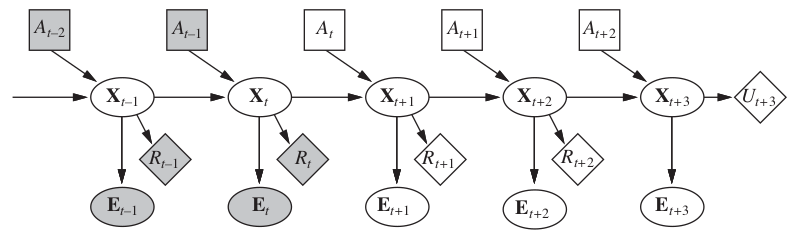
\includegraphics[width=10cm]{images/dynamic-decision-network.png}
    \caption{The generic structure of a dynamic decision network. Variables with known values are shaded. The current time is $t$ and the agent must decide what to do --- that is, choose a value for $A_t$ . The network has been unrolled into the future for three steps and represents future rewards, as well as the utility of the state at the look-ahead horizon.}
\end{figure}

In a DBN, the single state $S_t$ becomes a set of state variables $X_t$, along with possibly multiple evidence variables $E_t$. The action at time $t$ is referred to as $A_t$, giving the transition model as $P(X_{t+1})|X_t, A_t$ and the sensor model $P(E_t|X_t)$. We use $R_t$ to refer to the reward at time $t$ and $U_t$ the utility of $S_t$.\\

POMDP solvers need to solve 2 problems: Belief tracking, which is to determine the current belief given the history observed so far, and the planning problem, what the optimal action to take is given the current belief.\\

Solving the belief tracking problem is equivalent to solving the inference problem in the Bayesian network. Very often, exact inference is computationally intractable. Instead, it may be more feasible to perform approximate inference.\\

We can again use online search as seen before to solve the planning problem, where the state space in the case of POMDP now is uncountable.\\

In the case of the planning problem, the size of the search tree of depth $d$ for the POMDP is $O(|A|^d|E|^d)$, since for each action $a$ that is taken we have possibly $|E|$ evidence that be observed. For such a online search tree, we can employ the use of MCTS and UCT that we have seen before to approximate the utility of states. This is also known as POMCP. To run UCT on POMDPs using POMCP, we need to represent the beliefs in the form of nodes. Unlike the case in MPDs wherein we used states, it is difficult to generate belief states due to the uncountable number of them. As such, instead of propagating beliefs forward in trials, POMCP instead samples a state at the root node from the initial belief, then runs the simulation using the state to generate action-observation history by sampling from the transition model $P(s'|s, a)$, as well as the observations $P(e|s')$.

\pagebreak
\section{Game Theory}

So far we have concentrated on making decisions in uncertain environments. However, it does not account for that situation where uncertainty is due to other agents and the decisions they make. In this section we study the aspects of \textbf{game theory} that analyze games with simultaneous moves and other sources of partial observability.

\subsection{Single-Move Games}

We start by considering a restricted set of games; Ones where all players take actions simultaneously. A single-move game is defined by three components:

\begin{itemize}
    \item \textbf{Players} or agents who will be making decisions.
    \item \textbf{Actions} that the players can choose. Different players may not have the same set of actions available
    \item A \textbf{payoff function} that gives the utility to each player for each combination of actions
\end{itemize}

Each player in a game must adopt and then execute a \textbf{strategy} which analogous to policies but in the context of game theory. A \textbf{pure strategy} is a deterministic policy; For a single-move game, a pure strategy is just a single action. For many games an agent can do better with a \textbf{mixed} strategy which is a randomized policy that selects actions according to probability distributions defined over the actions. A \textbf{strategy profile} is an assignment of a strategy to each player. Given a strategy profile, the game's outcome is a numeric value for each player.\\

A solution to a game is a strategy profile in which each player adopts a rational strategy. This notion of rationality can be explained by the notion of \textbf{dominance}. We say that strategy $s$ for a player $p$ is a \textbf{strongly dominant strategy} if the outcome for $s$ is better for $p$ than the outcome for any other strategy $s'$, for every choice of strategies by the other player(s). Strategy $s$ \textbf{weakly dominates} $s'$ if $s$ is better than $s'$ on at least one strategy profile, and not worse on any other. A dominant strategy is one that dominates all others, and provides the best utility for player $p$ barring all other considerations. Hence, rationality implies that the dominant strategy be picked.\\

When each player has a dominant strategy, the combination of these strategies in one profile is known as the \textbf{dominant strategy equilibrium}. The definition of an equilibrium is where no player can benefit from switching his/her strategy, holding all other strategies by other players constant. This is also known as a \textbf{Nash equilibrium}, and a dominant strategy equilibrium is indeed a Nash equilibrium.\\

However, it is not always that the Nash equilibrium is the best possible outcome that is reached by all players. This is especially prevalent in the prisoner's dilemma. We see that if a player does not pick the dominant strategy, the player is not being rational and getting the best rewards possible, \textit{but only in the case where all other players do not change their strategy}. In some cases, a combination of players picking non-dominant strategies that may result in a better outcome that the one yield by the Nash equilibrium. We say that such an outcome is \textbf{Pareto dominating} since it it preferred by all players over the current one. An outcome is \textbf{Pareto optimal}, if it Pareto dominates all other outcomes. That is, it is the best outcome possible for the group.\\

While there is \textit{always a Nash equilibrium}, there may not always be a dominant strategy profile. Consider the game where there are no dominant strategy profiles, and two Nash equilibria. If both players aimed for different equilibria, then the overall utility of both agents would suffer! In such \textbf{coordination games}, agents are encouraged to communicate to reach a Pareto optimal solution which benefits that both.\\

A game can have more than one Nash equilibrium, and always has a Pareto Optimal outcome. But, they do not always have a \textit{pure-strategy} Nash equilibrium. Instead, we will have to look to \textit{mixed} strategies instead. In particular, we shall look at a method for computing an optimal mixed strategy in zero-sum games where utilities are shared between players(the utility of MAX player is the utility of the MIN player), which is known as the \textbf{minimax} or \textbf{maximin} technique. The brief outline of how this works is as follows:

\begin{enumerate}
    \item The first player(MAX player) can first reveal his strategy $[p, a_1; 1-p, a_2]$ to the opponent the MIN player. The MIN player, knowing the MAX player's strategy, can decide on the action that minimizes the expected utility according to this strategy. In this step, the MIN player always picks a deterministic or pure strategy, since the convex combination from a strategy $[q, a_1; 1-q, a_2]$ gives expected utility $q\cdots u_{a_1} + (1-q)\cdot u_{a_2} \geq \min(u_{a_1}, u_{a_2})$. This is similar to the minimax algorithm applied in two-player games.\\
    
    \item Then, we can simply choose a value $p$ for the mixed strategy of MAX player such that the outcomes of both actions $a_1, a_2$ by the MIN player yields the same utility. Then, the MIN player is indifferent to either actions and outcomes. Notice that this is the intersection point between the two expressions given by the utilities of both outcomes. This is the best at MAX can do, if not MIN player can always select an action that lowers the utility. Hence, the namesake minimax since the MAX player is trying to maximize the minimum utility it can get due to the MIN player's choice.\\
\end{enumerate}

Additionally, we can reverse the order as well: Letting the MIN player start first, then deriving the probability $q$ that yields MIN player lowest possible utility, given the choices of the MAX player after. What is interesting is that the true utility obtained in both orders are equivalent: That is, the max possible utility for the MAX player if he starts first, is equivalent to the minimum possible utility for the MIN player. We can see that a consequence of the minimax technique is that \textit{for every two player zero sum game, there is a maximin equilibirium when mixed strategies are allowed}. Furthermore, by the \textbf{minimax Theorem} from von Neumann:

\begin{theorem}
\text{\normalfont \textbf{Minimax}(von Neumann)}: Let $x$ and $y$ be the probability vectors representing the mixed strategies of MAX and MIN, and $A$ be the payoff matrix of MAX. The utility of the game is computed as $x^TAy$, and has the following property:

$$
\max_x \min_y x^TAy = \min_y \max_x x^TAy = v
$$

where $v$ is the utility of the game.
\end{theorem}

This implies that the maximin strategy for MIN is equivalent to the minimax strategy for MAX, as they give the same utility regardless of order. 

\subsection{Repeated Games}

So far, we have only looked at games which last a single move. The simplest kind of multiple-move game is the \textbf{repeated game}, in which players face the same choice repeatedly but each time with knowledge of the history of all player's previous choices. A strategy profile for a repeated game now specifies an action choice for each player at each time step for every possible history of previous choices. As with MDPs, we consider payoffs to be additive with discounts over time.\\

In a finite repeated game, surprisingly it not so different from a single move game. We can solve such games using \textbf{backward induction}. First consider that last game in the sequence. Since both players know that there can be no game after that, they will play a dominant strategy. Now that we have figured out the strategy profile for the last game, we move onto the second last one. But since the last game has already been determined, the second last game does not influence future games and both players again play the dominant strategy. We propagate such arguments backward for each game until the first to find that at the every first game and all games after, the players will not play any differently from a single-move game.\\

Instead, we consider a different version where the game is repeated at a probability of $p$. Then, there can only be a notion of the \textit{expected} number of rounds, but not a guarantee on which round the game truly ends. Under such conditions, more cooperative behaviours may be forced. Consider the prisoner's dilemma scenario, with $p=99$ which gives an expected number of rounds to be 100. The Nash equilibrium for the prisoner's dilemma occurs when either prisoners \textit{testify}, or both \textit{refuses}. Different choices for both leads to worse rewards for the one who \textit{refuses}. If both players continue to \textit{refuse}, then the payoffs for both players are

$$
\sum^{\infty}_{t=0} 0.99^t \cdot (-1) = -100
$$

However, one prisoner may deviate from this assumed strategy of always refusing to testify. In such cases, the other prisoner can adopt the \textbf{perpetual punishment} strategy which switches from \textit{refuse} to \textit{testify}. This results in the prisoner that initially testified to get a reward of 0, but be 'punished' every round after which yields the following utility

$$
0 + \sum^{\infty}_{1} 0.99^t \cdot (-1) = -495
$$

which aims to deter both prisoners from deviating. Of course, this would only work if both prisoners know that the other adopts the perpetual punishment strategy. Another strategy which works rather well in practice is the \textit{ti-for-tat}, where the player starts with an arbitrary move, and copies the other player's previous move for all rounds after.

\subsection{Sequential Games}

In the general case, a game that consists of a sequence of turns can be represented by a game tree which is also known as an \textbf{extensive form}, where the terminal nodes consist of payoffs to each player. Each non-terminal node is allocated to a particular player and is a decision node where the edges consists of actions the player can make. To represent uncertainty arising from the environment or the player's actions, we introduce an arbitrary player represented by \textit{chance nodes}.\\

In game trees representing sequences of turns, the Minimax algorithm cannot handle cases where there is partial observability, such as unknown information from other players. This is one of the differences between extensive forms and game trees used in the Minimax algorithm, where it is able to handle imperfect information by defining \textbf{information sets}. Information sets are a set of nodes that belongs to the same player with the same observation history. The player may not be able to distinguish which node it belongs to based on what the player has observed so far. A visual representation of a game tree can be seen below:

\begin{figure}
    \centering
    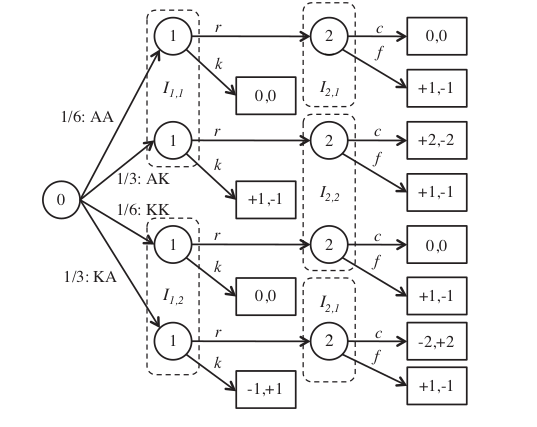
\includegraphics[width=10cm]{images/sequential_gt.png}
    \caption{Extensive form of a simplified version of poker.}
    \label{fig:sgt}
\end{figure}

One way to solve an extensive game is to convert it to a normal-form game as seen before. Then, each row and column represents actions taken by both players with the corresponding value representing the payoffs seen in terminal nodes. An issue with such solutions is that given $I$ information sets and $a$ actions, then there are $a^I$ possible strategies for a single player.\\

In a game tree, each subtree in the game tree also represents a subgame. If each of these subgames in the game tree are at equilibrium, then we say that the Nash equilibrium achieved is a \textbf{subgame perfect Nash equilibrium}. 

\end{document}  